%%%%%%%%%%%%%%%%%%%%%%%%%%%%%%%%%%%%%%%%%%%%%%%%%%%%%%%%%%%%%%%%%%%%%%%%%%%%%%%
% Author:  Pablo Alvarado
%
% Escuela de Ingeniería Electrónica
% Instituto Tecnológico de Costa Rica
%
% Tesis de Licenciatura
% 
% Phone:   +506 2550 9005
% email:   palvarado@itcr.ac.cr
%
%%%%%%%%%%%%%%%%%%%%%%%%%%%%%%%%%%%%%%%%%%%%%%%%%%%%%%%%%%%%%%%%%%%%%%%%%%%%%%%

% \documentclass is book
% If you want a printable two-side version of the thesis
%\documentclass[12pt,twoside,letterpaper]{book}

% If you want an electronic-only version of the thesis, do it one-sided
\documentclass[12pt,oneside,letterpaper]{book}

\usepackage[T1]{fontenc}
%\usepackage[utf8]{inputenc}   % is no longer required (since 2018)
\usepackage{ifthen}            % provide if-then-else operators

% --------------------------------------------------------------------------
% Global variables required in document formatting
% --------------------------------------------------------------------------
%
% BOOK MODE
%
\newboolean{bookmode}                  % boolean used to control book format
% Ensure that only one of the next two lines is active:
\setboolean{bookmode}{true}           % turn book mode on
%\setboolean{bookmode}{false}           % turn book mode off

%
% DRAFT MODE
%   The draft mode activates the TODO index and some "draft" markings all
%   around.  Ensure you set it to false for the final version!!
%   
%
\newboolean{draftmode}                  % boolean used to control draft-mode

%% -------------------------------------------------------------------------

%% Configure su nombre, título de tesis, lectores, fechas, etc. en:
%%
%% >>>>  config.tex  <<<<
%%

% --------------------------------------------------------------------------

% include all packages and define all required general macros
%%%%%%%%%%%%%%%%%%%%%%%%%%%%%%%%%%%%%%%%%%%%%%%%%%%%%%%%%%%%%%%%%%%%%%%%%%%%%%%
% Author:  Pablo Alvarado
%
% Escuela de Electrónica
% Instituto Tecnológico de Costa Rica
%
% Phone:   +506 2550 9005
% email:   palvarado@itcr.ac.cr
% 
%%%%%%%%%%%%%%%%%%%%%%%%%%%%%%%%%%%%%%%%%%%%%%%%%%%%%%%%%%%%%%%%%%%%%%%%%%%%%%%

\PassOptionsToPackage{usenames,dvipsnames}{xcolor}

% -----------------------------------------------------------------------------
%   Define all configuration commands
% -----------------------------------------------------------------------------

\newcommand{\genderLector}[1]{%
  \ifthenelse{\equal{#1}{F}}{%
    Profesora Lectora%
  }{%
    \ifthenelse{\equal{#1}{M}}{%
      Profesor Lector%
    }{%
      Persona profesora lectora%
    }%
  }%
}

% Lector I
\newcommand{\nameLectorI}{$<$\emph{Use defLectorI in config.tex}$>$}
\newcommand{\genderLectorI}{N/A}

\newcommand{\defLectorI}[1][M]{%
  \renewcommand{\genderLectorI}{\genderLector{#1}}%
  \lectorIRelay%
}

\newcommand{\lectorIRelay}[1]{%
  \renewcommand{\nameLectorI}{#1}
}

%% Lector II
\newcommand{\nameLectorII}{$<$\emph{Use setLectorII in main.tex}$>$}
\newcommand{\genderLectorII}{N/A}

\newcommand{\defLectorII}[1][M]{%
  \renewcommand{\genderLectorII}{\genderLector{#1}}%
  \lectorIIRelay%
}

\newcommand{\lectorIIRelay}[1]{%
  \renewcommand{\nameLectorII}{#1}
}

%% Asesor
\newcommand{\nameAsesor}{$<$\emph{Use setAsesor in main.tex}$>$}
\newcommand{\genderAsesor}{$<$\emph{Use setAsesor in main.tex}$>$}

\newcommand{\defAsesor}[1][M]{%
  \ifthenelse{\equal{#1}{F}}{%
    \renewcommand{\genderAsesor}{Profesora Asesora}%
  }{%
    \ifthenelse{\equal{#1}{M}}{%
      \renewcommand{\genderAsesor}{Profesor Asesor}%
    }{%
      % La RAE no ha definido cómo hacer esto...
      %
      % Hay que preguntar a la persona asesora no-binaria directamente
      % cómo gusta ser tratada.
      \renewcommand{\genderAsesor}{Persona profesora asesora}%
    }
  }
  \asesorRelay
}

\newcommand{\asesorRelay}[1]{%
  \renewcommand{\nameAsesor}{#1}
}

% Dates for draft and final
\newcommand{\thesisDraftDate}{\today}
\newcommand{\defDraftDate}[1]{\renewcommand{\thesisDraftDate}{#1}}

\newcommand{\thesisFinalDate}{$<$\emph{Fecha de Defensa en config.tex}$>$}
\newcommand{\defFinalDate}[1]{\renewcommand{\thesisFinalDate}{#1}}

% Author definition and gender related strings

\newcommand{\thesisAuthor}{Error: Undefined}
\newcommand{\thesisAuthorShort}{Error: Undefined}
\newcommand{\thesisAuthorTECID}{Error: Undefined}
\newcommand{\thesisAuthorAddress}{Error: Undefined}
\newcommand{\thesisAuthorDegree}{Error: Undefined}

\newcommand{\defAuthor}[1][M]{%
  \ifthenelse{\equal{#1}{F}}{%
    \renewcommand{\thesisAuthorAddress}{la señora}
    \renewcommand{\thesisAuthorDegree}{Ingeniera}
  }{%
    \ifthenelse{\equal{#1}{f}}{%
      \renewcommand{\thesisAuthorAddress}{la señorita}
      \renewcommand{\thesisAuthorDegree}{Ingeniera}
    }{%
      \ifthenelse{\equal{#1}{M}}{%
        \renewcommand{\thesisAuthorAddress}{el señor}
        \renewcommand{\thesisAuthorDegree}{Ingeniero}
        
      }{%
        \renewcommand{\thesisAuthorAddress}{la persona}
        \renewcommand{\thesisAuthorDegree}{Ingeniere}
      }
    }
  }
  \authorRelay
}

\newcommand{\authorRelay}[1]{%
  \renewcommand{\thesisAuthor}{#1}
}

\newcommand{\defAuthorShort}[1]{%
  \renewcommand{\thesisAuthorShort}{#1}
}

\newcommand{\defAuthorTECID}[1]{%
  \renewcommand{\thesisAuthorTECID}{#1}
}

%% About the institution and department
\newcommand{\thesisDepartment}{Escuela de Ingeniería Electrónica}
\newcommand{\thesisInstitution}{Tecnológico de Costa Rica}

\newcommand{\defDepartment}[1]{%
  \renewcommand{\thesisDepartment}{#1}
}

\newcommand{\defInstitution}[1]{%
  \renewcommand{\thesisInstitution}{#1}
}



%% About the report name, and type
\newcommand{\thesisTitle}{Error: Undefined}
\newcommand{\thesisFlatTitle}{\thesisTitle}
\newcommand{\thesisKeywords}{Error: Undefined}
\newcommand{\thesisType}{Error: Undefined}

%% A tool to remove new lines leaving no spaces
\newcommand\titleFlattener[1]{\def\\{\relax\ifhmode\unskip\fi\space\ignorespaces}#1}

\newcommand{\defTitle}[1]{%
  \renewcommand{\thesisFlatTitle}{\titleFlattener{#1}}
  \renewcommand{\thesisTitle}{#1}
}

\newcommand{\defKeywords}[1]{%
  \renewcommand{\thesisKeywords}{#1}
}

\newcommand{\defTFGType}[1]{%
  \renewcommand{\thesisType}{#1}
}

%% Este archivo contiene toda la configuración básica del documento de
%% tesis, para centralizar alguna información que se requiere en todo
%% el documento.

%% DRAFT MODE

%%   El modo borrador activa las listas de cosas por hacer, con su
%%   índice, y algunas marcas explícitas de "borrador" por todo lado.
%%
%%   Asegúrse de que esta variable sea false en la versión final y de haber
%%   actualizado la fecha de la defensa, un poco más abajo.
\setboolean{draftmode}{true}            % turn draft mode on
%\setboolean{draftmode}{false}          % turn draft mode off

%% Esta es la fecha que se colocará en el modo borrador
\defDraftDate{\today}
%% Esta es la fecha que se usará en la versión final
\defFinalDate{28 de noviembre, 2025}

%% Este es el nombre del estudiante y el pronombre que utiliza, para cambiar
%% las portadas como corresponde

% Con el nombre de autor, se debe especificar el género a utilizar:
%
%   [M]asculino
%   [F]emenino (usando "señora" donde corresponda)
%   [f]emenino (usando "señorita" donde corresponda)
%   persona [N]o binaria
%
%   Debido a la falta de norma en español para las personas no binarias,
%   posíblemente deba ajustarse para el gusto de cada quien.
%
\defAuthor[M]{Justin Jaffeth Corea Masis}                % Nombre del estudiante
%\defAuthor[f]{María del Pilar Pérez Prado}    % Nombre de la estudiante

\defAuthorShort{J.~Corea}                      % Nombre corto
\defAuthorTECID{2020045294}                     % Carné

%% Este es el título completo del informe del trabajo final de graduación.
%% Usted puede agregar \\ para forzar líneas nuevas en la portada y automática-
%% mente el comando se encarga de eliminar eso cuando necesita el título
\defTitle{Reconocimiento automático de números de placas\\
  para la gestión automática de estacionamientos \\%
  en el Campus Tecnológico Local San José}

%% Palabras clave
\defKeywords{ANPR, end-to-end, YOLOv11, IPLMS, Sintético}

%% Tribunal Evaluador
%%
%% Indique los nombres de los lectores y asesor
%% El parámetro opcional es
%%  [M]asculino,
%%  [F]emenino,
%%  persona [N]o binaria
\defLectorI[M]{Ing.\,Javier Mauricio Perez Rodriguez}
\defLectorII[M]{Ing.\,Sergio Alberto Ariola Valverde} 
\defAsesor[M]{Dr.\,Jose Pablo Alvarado Moya}

%% Tipo de tesis o informe
%%   - Tesis de Licenciatura
%%   - Informe de Proyecto Final 
%%   - Tesis de Maestría
\defTFGType{Tesis de Licenciatura}

%% Nombre del departamento e institución
\defInstitution{Instituto Tecnológico de Costa Rica}
\defDepartment{Escuela de Ingeniería Electrónica}

 % Load the desired configuration

%Para el PDF (cambiar si se desea otras cosas a lo indicado arriba
\newcommand{\pdfAuthor}{\thesisAuthor}
\newcommand{\pdfTitle}{\thesisFlatTitle} 
\newcommand{\pdfKeywords}{\thesisKeywords}
\newcommand{\pdfSubject}{\thesisType}


%% -------------------------------------------------------------------

\usepackage{ifpdf}

% Command to change between draft or release mode:
\newcommand{\ifdraft}[2]{\ifthenelse{\boolean{draftmode}}{#1}{#2}}
% Command to change between draft or release mode:
\newcommand{\ifbook}[2]{\ifthenelse{\boolean{bookmode}}{#1}{#2}}

% include all required packages here
\usepackage{comment}
\usepackage{float}
\usepackage{csquotes}                  % recommended for biblatex
\usepackage[american,spanish,es-tabla]{babel}   % spanish, remove es-tabla for cuadro
%\usepackage[spanish]{babel}   % spanish, remove es-tabla for cuadro

\usepackage{xspace} % Decide if a space is needed at the end of some commands

\makeatletter
% babel uses a hook and therefore the tablename is here not defined yet.
% However, it defines es@tablename with upper/lowercase, and we use it.
\ifthenelse{\equal{\es@tablename}{Ttabla}}{%
  \newcommand{\cuadro}{tabla}
  \newcommand{\cuadros}{tablas}
  \newcommand{\Cuadro}{Tabla}
  \newcommand{\elcuadro}{la tabla}
  \newcommand{\Elcuadro}{La tabla}
  \newcommand{\loscuadros}{las tablas}
  \newcommand{\Loscuadros}{Las tablas}
  
  \newcommand{\tabla}{tabla}
  \newcommand{\tablas}{tablas}
  \newcommand{\Tabla}{Tabla}
  \newcommand{\latabla}{la tabla}
  \newcommand{\Latabla}{La tabla}
  \newcommand{\lastablas}{las tablas}
  \newcommand{\Lastablas}{Las tablas}
  
  \newcommand{\tabref}[1]{\hyperref[#1]{tabla~\ref*{#1}}\xspace}
  \newcommand{\Tabref}[1]{\hyperref[#1]{Tabla~\ref*{#1}}\xspace}

  \newcommand{\latabref}[1]{la \tabref{#1}}
  \newcommand{\Latabref}[1]{La \tabref{#1}}

}{%
  \newcommand{\cuadro}{cuadro}
  \newcommand{\cuadros}{cuadros}
  \newcommand{\Cuadro}{Cuadro}
  \newcommand{\elcuadro}{el cuadro}
  \newcommand{\Elcuadro}{El cuadro}
  \newcommand{\loscuadros}{los cuadros}
  \newcommand{\Loscuadros}{Los cuadros}
  
  \newcommand{\tabla}{cuadro}
  \newcommand{\tablas}{cuadros}
  \newcommand{\Tabla}{Cuadro}
  \newcommand{\latabla}{el cuadro}
  \newcommand{\Latabla}{El cuadro}
  \newcommand{\lastablas}{los cuadros}
  \newcommand{\Lastablas}{Los cuadros}
  
  \newcommand{\tabref}[1]{\hyperref[#1]{cuadro~\ref*{#1}}\xspace}
  \newcommand{\Tabref}[1]{\hyperref[#1]{Cuadro~\ref*{#1}}\xspace}

  \newcommand{\latabref}[1]{el \tabref{#1}}
  \newcommand{\Latabref}[1]{El \tabref{#1}}

}
\makeatother

% References to figures
\newcommand{\figref}[1]{\hyperref[#1]{figura~\ref*{#1}}\xspace}
\newcommand{\Figref}[1]{\hyperref[#1]{Figura~\ref*{#1}}\xspace}
\newcommand{\lafigref}[1]{la \hyperref[#1]{figura~\ref*{#1}}\xspace}
\newcommand{\Lafigref}[1]{La \hyperref[#1]{figura~\ref*{#1}}\xspace}

% References to equations
\newcommand{\equ}[1]{\hyperref[#1]{(\ref*{#1})}\xspace}

% Refrences to chapters and sections
\newcommand{\capref}[1]{\hyperref[#1]{capítulo~\ref{#1}}\xspace}
\newcommand{\secref}[1]{\hyperref[#1]{sección~\ref{#1}}\xspace}

\usepackage{makeidx}                    % to create index file

\usepackage[nottoc]{tocbibind}          % Fix the hyperrefs to TOC,TOF, etc.
                                        % and ensure that they appear all in 
                                        % the Table of Contents
\ifdraft{%
  %\usepackage[refpage]{nomencl}        % Use to easily administrate the list
  \usepackage[intoc,spanish]{nomencl}   % of symbols
}{%
  \usepackage[intoc,spanish]{nomencl}
}

\usepackage{siunitx}                    % Units of the SI
\sisetup{output-decimal-marker = {,}}   % Use decimal , instead of decimal .
\DeclareSIQualifier\peak{p}
\DeclareSIQualifier\ppeak{pp}

\usepackage{amsmath}
\usepackage{amssymb,amstext}            % AMS-math and symbols package
\usepackage{mathrsfs}                   % Calygraphic fonts for transforms
\usepackage{trsym}                      % Para símbolos de transformadas o---o
\usepackage{stmaryrd}                   % For short arrows
\usepackage{nicefrac}
\usepackage{array}                      % extensions to tabular environment
\usepackage{longtable}                  % supports extraordinary long tables
\usepackage{tabularx}                   % supports tables with fixed width

\usepackage[backend=biber,              % Use biber/biblatex
            style=ieee,
            sorting=none,
            citestyle=numeric-comp]{biblatex}

\usepackage{afterpage}                  % put something only after the page
\usepackage{multirow}                   % supports multiple row grouping in 
                                        % tables
\usepackage{multicol}                   % multiple columns environments
\usepackage{enumitem}                   % better enumeration with paralist 
                                        % equivalents as follows:

\newlist{compactitem}{itemize}{3}
\setlist[compactitem]{topsep=0pt,partopsep=0pt,itemsep=0pt,parsep=0pt}
\setlist[compactitem,1]{label=\textbullet}
\setlist[compactitem,2]{label=---}
\setlist[compactitem,3]{label=*}

\newlist{compactdesc}{description}{3}
\setlist[compactdesc]{topsep=0pt,partopsep=0pt,itemsep=0pt,parsep=0pt}

\newlist{compactenum}{enumerate}{3}
\setlist[compactenum]{label*=\arabic*.,topsep=0pt,partopsep=0pt,itemsep=0pt,parsep=0pt}
\newlist{compactenuma}{enumerate}{3}
\setlist[compactenuma]{label*=\alph*.,topsep=0pt,partopsep=0pt,itemsep=0pt,parsep=0pt}

\usepackage{icomma}                     % decimal comma in math mode

\usepackage{bold-extra}

\usepackage[format=hang,%
            font=small,%
            labelfont=bf]{caption}      % nicer figure captions
\usepackage{subcaption}                 % for subfigures
            
\usepackage{booktabs}                   % book type tabulars
\usepackage{pdfpages}                   % used to include the final "acta"

% the own style with options depending on the draft mode
\ifdraft{%
\usepackage[todo]{sty/tecStyle}         % some command definitions
                                        % options [todo] todo-index
}{%
\usepackage{sty/tecStyle}               % some command definitions
                                        % options [todo] todo-index
}

%% fix the title for examples
\renewcommand{\examplelistname}{Índice de ejemplos}
\renewcommand{\examplename}{Ejemplo}

%% define some command to cope with the tribunal names

%% Lector I


\usepackage{url}                        % allows linebreaks at certain
                                        % characters or combinations of 
                                        % characters for URLs

%% Usual tikz libraries and configuration
\usepackage{tikz}
\usepackage{pgfplots}
\pgfplotsset{compat=1.16}
\usepgfplotslibrary{fillbetween}
\usetikzlibrary{patterns,shapes,arrows.meta,positioning,calc,babel}
\usetikzlibrary{fit,shapes.geometric,decorations.markings}

\usepackage{listings}                   % syntax highlighting of code fragments

\lstdefinestyle{verilog-style}
{
  language=Verilog,
  basicstyle=\small\ttfamily,
  keywordstyle=\color{dkblue},
  identifierstyle=\color{black},
  commentstyle=\color{dkgreen},
  numbers=left,
  numberstyle=\tiny\color{black},
  numbersep=10pt,
  tabsize=8,
  moredelim=*[s][\colorIndex]{[}{]},
  literate=*{:}{:}1
}
\lstset{literate=%
  {á}{{\'a}}1
  {é}{{\'e}}1
  {í}{{\'i}}1
  {ó}{{\'o}}1
  {ú}{{\'u}}1
  {ñ}{{\~n}}1
  {Á}{{\'A}}1
  {É}{{\'E}}1
  {Í}{{\'I}}1
  {Ó}{{\'O}}1
  {Ú}{{\'U}}1
  {Ñ}{{\~N}}1
}

\definecolor{vorange}{RGB}{255,143,102}

\makeatletter
\newcommand*\@lbracket{[}
\newcommand*\@rbracket{]}
\newcommand*\@colon{:}
\newcommand*\colorIndex{%
    \edef\@temp{\the\lst@token}%
    \ifx\@temp\@lbracket \color{black}%
    \else\ifx\@temp\@rbracket \color{black}%
    \else\ifx\@temp\@colon \color{black}%
    \else \color{vorange}%
    \fi\fi\fi
}
\makeatother


% For pdflatex
% - The hyperref package should always be loaded last, since it has to
%   overwrite some of the commands.
% - The package subfigure caused that the pagebackrefs and index refs were set
%   incorrectly.

\ifpdf
%
% final / draft document options
%\usepackage{graphicx}                   % for inserting pdf-graphics.
                                        % options final / draft
\ifdraft{%
\usepackage[%pdftex,%
            naturalnames=true,
            linktocpage,
            hyperindex,
            colorlinks,
            urlcolor=dkred,          %\href to external url
            filecolor=dkmagenta,     %\href to local file
            linkcolor=dkred,         %\ref and \pageref
            citecolor=dkgreen,       %\cite
            plainpages=false,
            pdfpagelabels,
            pdfpagemode=UseOutlines, % means use bookmarks (None,UseOutlines)
            % bookmarksopen=false,   % would show the whole hierarchy if true
            bookmarksnumbered=true,
            pdfpagelayout=OneColumn, % SinglePage,OneColumn,TwoColumnLeft,...
            pdfview=FitH, % FitB,FitBH,FitBV,Fit,FitH,FitV
            pdfstartview=FitH, % FitB,FitBH,FitBV,Fit,FitH,FitV
            unicode,
            ]{hyperref}
}{%
% Use biber/biblatex
\usepackage[%pdftex,%
            naturalnames=true,
            linktocpage,hyperindex,
            colorlinks,
            urlcolor=dkred,          %\href to external url
            filecolor=dkmagenta,     %\href to local file
            linkcolor=dkred,         %\ref and \pageref
            citecolor=dkgreen,       %\cite
            plainpages=false,
            pdfpagelabels,
            pdfpagemode=UseOutlines, % means use bookmarks (None,UseOutlines)
            % bookmarksopen=false,   % open the whole hierarchy if true!
            bookmarksnumbered=true,
            pdfpagelayout=OneColumn, % SinglePage,OneColumn,TwoColumnLeft,...
            pdfview=FitH, % FitB,FitBH,FitBV,Fit,FitH,FitV
            pdfstartview=FitH, % FitB,FitBH,FitBV,Fit,FitH,FitV,
            unicode,
            ]{hyperref}
}


%
% Ensure that the links of the images point to the top of the images and not
% to the caption
%
\usepackage[figure]{hypcap}

% %
% % Ensure that pdfLaTeX do the same spacing as LaTeX
% %
\pdfadjustspacing=1 
% %
\else   % i.e. if not pdf

\usepackage[active]{srcltx}             % insert links into the dvi to jump
\usepackage{graphicx}                   % for inserting eps-graphics.
                                        % options final / draft
                                        % into the sources directly.
\ifdraft{%
\usepackage[ps2pdf,%
            % plainpages=false,
            linktocpage,
            hyperindex,
            % pdfpagelabels,
            pdfpagemode=UseOutlines,
            pdfstartview=FitH,
            unicode,]{hyperref}
}{%
\usepackage[ps2pdf,%
            % plainpages=false,
            linktocpage,
            hyperindex,
            % pdfpagelabels,
            pdfpagemode=UseOutlines,
            pdfstartview=FitH,
            unicode,]{hyperref}
}

%\usepackage[ps2pdf]{hyperref}

\fi  % end of if pdf or not

% --------------------------------------------------------------------------

% Allow the use of international characters
\AtBeginDocument{%
  \hypersetup{%
             pdftitle={\pdfTitle},%
             pdfsubject={\pdfSubject},%
             pdfauthor={\pdfAuthor},%
             pdfkeywords={\pdfKeywords}
            }%
}


%\usepackage{algorithmic}            % algorithmic environment


\usepackage{rotating}                % allow block rotation

%% This environment will allow to rotate a page in the PDF, just
%% for visualization purposes.  Since nowadays the documents are
%% almost never printed, it is best if rotated pages are also shown
%% rotated in the PDF viewer, and this is the purpose of this environment.
\newenvironment{rotatepage}%
{\global\pdfpageattr\expandafter{\the\pdfpageattr/Rotate 90}}%
{\clearpage\pagebreak[4]\global\pdfpageattr\expandafter{\the\pdfpageattr/Rotate 0}}

    
%%%%%%%%%%%%%%%%%%%%%%%%%%%%%%%%%%%%%%%%%%%%%%%%%%%%%%%%%%%%%%%%%%%%%%%%%%%%%%%

%\sloppy

%
% Some own font definitions
%
\DeclareMathAlphabet{\mathpzc}{OT1}{pzc}{m}{it}
\DeclareMathAlphabet{\mathpss}{OT1}{cmss}{m}{sl}

%
% page layout
%

\usepackage{vmargin}
\setpapersize{USletter}

% For letter-paper printing
\setmarginsrb{33mm}{8mm}{23mm}{7mm}{15pt}{15pt}{7mm}{12mm}
%\setlength{\headheight}{15pt}         % fancy headers wanted this

%
% Fraction of Float Object / Text
%

\renewcommand{\topfraction}{0.95}       % how much of top of page should be 
                                        % allowed to be float object?
\renewcommand{\bottomfraction}{0.95}    % how much of bottom of page should be
                                        % allowed to be float object?
\renewcommand{\textfraction}{0.05}      % how much of page must be text?

\usepackage{fancyhdr}                   % fancy page headers

\usepackage{lastpage}

%
% header and footer layout (needs package fancyhdr)
%
\newcommand{\copyrightfooter}{\tiny{\copyright \the\year\ --- \thesisAuthorShort %
    \qquad Uso exclusivo ITCR}}
%
\newcommand{\draftfoot}%
  {\ifdraft{\textcolor{dkblue}{\tiny\textsl{Borrador: \today}}{}}
           {}
}

\pagestyle{fancy}
\renewcommand{\chaptermark}[1]{\markboth{{\small
    \thechapter\hspace*{1mm}#1}}{}}
\renewcommand{\sectionmark}[1]{\markright{{\small
    \thesection\hspace*{1mm}#1}}{}}
%\lhead[{\small\textsc\Roman{\thepage}}]{\fancyplain{}%
\lhead[{\small\thepage}]{\fancyplain{}%
        {{\slshape \small\nouppercase{\leftmark}}}}
\chead[]{}
\rhead[\fancyplain{}%
%        {{\slshape \small\nouppercase{\rightmark}}}]{{\small\textsc\Roman{\thepage}}}
        {{\slshape \small\nouppercase{\rightmark}}}]{{\small\thepage}}
\lfoot[]{\draftfoot}
\ifbook{%
  \cfoot[]{}
}{
  \cfoot[\copyrightfooter]{\copyrightfooter}
}
\rfoot[\draftfoot]{}
\renewcommand{\headrulewidth}{0.5pt}
\renewcommand{\footrulewidth}{0pt}

%
% Caption style for tables
% For caption v3:
\captionsetup[table]{position=top,
  format=hang,
  textfont={normalsize},
  labelfont={normalsize,bf}}

\newcommand{\tablecaption}[2][foo]{%
  \ifthenelse{\equal{#1}{foo}}{%
    \caption{#2}%
  }{%
    \caption[#1]{#2}%
  }
}

%% En español hay diferencia entre Tabla y Cuadro.
%%
%% Tabla: es la tabla periódica, o una tabla de logaritmos o de
%%        probabilidades o de integrales. Usualmente es algo que no
%%        requiere referencias o explicaciones adicionales en el texto porque
%%        todas sus entradas son sucesiones de alguna cosa que se busca allí
%%        mismo
%% Cuadro: es lo que usualmente se usa en inglés como "table", y resume
%%        información que requiere al menos parcialmente explicaciones en el
%%        el texto.

%% \addto\extrasspanish{\renewcommand{\tablename}{Tabla}}
%% \addto\extrasspanish{\renewcommand{\listtablename}{\'Indice de tablas}}

%
% paragraph layout
%
\renewcommand{\baselinestretch}{1.1}    % line spacing
\parindent0em                           % indentation width of first line
\parskip1.3ex                           % space between paragraphs

%
% document consists of
% chapter - section - subsection - subsubsection - paragraph - subparagraph
%
\setcounter{secnumdepth}{2}             % depth of section numbering
\setcounter{tocdepth}{2}                % depth of table of contents

% For biblatex
\addbibresource{literatura.bib}

%
% prepares index from entries like \index{word} or \index{group!word}.
% don't forget to call "makeindex filename" for final index generation.
%
\makeindex                            %% for package makeidx.sty
%\newindex{default}{idx}{ind}{Index}  %% for package index.sty

\newcommand{\octave}{GNU/Octave}
\newcommand{\linux}{GNU/Linux}


\newcommand{\placeholderimage}[1]{%
  \fbox{\parbox[c][0.6\linewidth][c]{#1}{\centering Placeholder}}%
}

%
% prepares notation or nomenclature 
%
\makenomenclature

%%% Local Variables: 
%%% mode: latex
%%% TeX-master: "main"
%%% End: 


% define all symbols used in the document
%% ---------------------------------------------------------------------------
%% paNotation.tex
%%
%% Notation
%%
%% $Id: notation.tex 1467 2010-07-24 16:47:17Z palvarado $
%% ---------------------------------------------------------------------------

\newcommand{\nms}{\negmedspace}

%%
% Command definitions for localized symbol format definition
%%
\renewcommand{\Re}{\operatorname{Re}}
\renewcommand{\Im}{\operatorname{Im}}

\newcommand{\prt}[1]{\ensuremath{\mathcal{#1}}}         %% partitioning
\newcommand{\img}[1]{\ensuremath{\mathcal{#1}}}         %% image as a set
\newcommand{\reg}[1][R]{\ensuremath{\mathcal{#1}}}      %% region
\newcommand{\pred}[1]{\ensuremath{\mathrm{#1}}}         %% predicate
\newcommand{\operat}[2]{\mathcal{#1}\left\{#2\right\}}
\newcommand{\transf}[1]{\mathscr{#1}}
\newcommand{\fourier}[1]{\transf{F}\left\{#1\right\}}
\newcommand{\ifourier}[1]{\transf{F}^{-1}\left\{#1\right\}}
\newcommand{\laplace}[1]{\transf{L}\left\{#1\right\}}
\newcommand{\ulaplace}[1]{\transf{L}_u\left\{#1\right\}}
\newcommand{\blaplace}[1]{\transf{L}_b\left\{#1\right\}}
\newcommand{\ilaplace}[1]{\transf{L}^{-1}\left\{#1\right\}}
\newcommand{\ztrans}[1]{\transf{Z}\left\{#1\right\}}
\newcommand{\iztrans}[1]{\transf{Z}^{-1}\left\{#1\right\}}
\newcommand{\zutrans}[1]{\transf{Z}_u\left\{#1\right\}}
\newcommand{\exceq}{\ensuremath{\overset{!}{=}}}

\newcommand{\signum}{\operatorname{signum}}
\newcommand{\vct}[1]{\ensuremath{\underline{\mathbf{#1}}}}
\newcommand{\mat}[1]{\ensuremath{\mathbf{#1}}}
\newcommand{\vctmu}{\vct{\boldsymbol{\mu}}}
\newcommand{\vctzeta}{\vct{\boldsymbol{\zeta}}}
\newcommand{\vctpi}{\vct{\boldsymbol{\pi}}}
\newcommand{\vctvarphi}{\vct{\boldsymbol{\varphi}}}
\newcommand{\raum}[1]{\ensuremath{\mathbb{#1}}}
\newcommand{\matSigma}{\mat{\boldsymbol{\Sigma}}}
\newcommand{\matLambda}{\mat{\boldsymbol{\Lambda}}}
\newcommand{\matPsi}{\mat{\boldsymbol{\Psi}}}
\newcommand{\matPhi}{\mat{\boldsymbol{\Phi}}}
\newcommand{\row}[2]{\ensuremath{\mathbf{\underline{#1}_{#2(\cdot)}}}}
\newcommand{\col}[2]{\ensuremath{\mathbf{\underline{#1}_{(\cdot) #2}}}}
\newcommand{\seq}[1]{\ensuremath{#1}}
\newcommand{\set}[1]{\ensuremath{\mathcal{#1}}}
\newcommand{\gset}[1]{\ensuremath{#1}} %% set for greek symbols
\newcommand{\front}[1]{\widehat{\set{#1}}}
\newcommand{\setlambda}{\set{\boldsymbol{\lambda}}}
\newcommand{\klass}[1]{\ensuremath{\mathpss{#1}}}
\newcommand{\graph}[1]{\ensuremath{\mathsf{#1}}}
\newcommand{\lab}[1]{\ensuremath{\mathpss{L}(#1)}}
\newcommand{\myfrac}[2]{{\footnotesize #1/#2}}
\newcommand{\ifthenspc}{\rule{3mm}{0mm}}
\newcommand{\point}[1]{\ensuremath{\mathsf{#1}}}
\newcommand{\estim}[1]{\ensuremath{\hat{#1}}}
\newcommand{\numset}[1]{\ensuremath{\mathbb{#1}}}
\newcommand{\tuple}[1]{\ensuremath{\left\langle#1\right\rangle}}
\newcommand{\norm}[1]{\ensuremath{\left\lVert#1\right\rVert}}
\newcommand{\conj}[1]{\ensuremath{{{#1}^{\ast}}}}
\newcommand{\base}[1]{\set{#1}}
\newcommand{\zeron}[1]{\ensuremath{\underset{\uparrow}{#1}}}
\newcommand{\sysT}{\ensuremath{\mathcal{T}}}
\newcommand{\sys}[1]{\ensuremath{\sysT\left[#1\right]}}
%\newcommand{\sen}{\operatorname{sen}} % sinus in spanish (seno)
%\newcommand{\senh}{\operatorname{senh}} % sinus hiperbolicus in spanish (seno)
%\newcommand{\arcsen}{\operatorname{arcsen}} % arcus sinus hiperbolicus in spanish (arcoseno)
\newcommand{\sgn}{\operatorname{sgn}} % signus
\newcommand{\roc}{\text{ROC: }}

\newcommand{\code}[1]{\texttt{#1}}
\newcommand{\conv}{\ensuremath{\ast}}
\newcommand{\cconv}{\ensuremath{\;\,\text{\footnotesize{N}}\!\!\!\!\!\!\bigcirc}}
\newcommand{\Ln}{\operatorname{Ln}}
\newcommand{\rand}{\operatorname{rand}}
\newcommand{\sa}{\operatorname{sa}}
\newcommand{\senc}{\operatorname{senc}}


%% Natural, Integer and Real Numbers
\newcommand{\setA}{\ensuremath{\mathbb{A}}}
\newcommand{\setB}{\ensuremath{\mathrm{I\negthinspace B}}}
\newcommand{\setC}{\ensuremath{\mathbb{C}}}
\newcommand{\setD}{\ensuremath{\mathrm{I\negthinspace D}}}
\newcommand{\setE}{\ensuremath{\mathrm{I\negthinspace E}}}
\newcommand{\setF}{\ensuremath{\mathrm{I\negthinspace F}}}
\newcommand{\setG}{\ensuremath{\mathbb{G}}}
\newcommand{\setH}{\ensuremath{\mathrm{I\negthinspace H}}}
\newcommand{\setI}{\ensuremath{\mathbb{I}}}
\newcommand{\setJ}{\ensuremath{\mathbb{J}}}
\newcommand{\setK}{\ensuremath{\mathrm{I\negthinspace K}}}
\newcommand{\setL}{\ensuremath{\mathrm{I\negthinspace L}}}
\newcommand{\setM}{\ensuremath{\mathrm{I\negthinspace M}}}
\newcommand{\setN}{\ensuremath{\mathrm{I\negthinspace N}}}
\newcommand{\setO}{\ensuremath{\mathbb{O}}}
\newcommand{\setP}{\ensuremath{\mathrm{I\negthinspace P}}}
\newcommand{\setQ}{\ensuremath{\mathbb{Q}}}
\newcommand{\setR}{\ensuremath{\mathrm{I\negthinspace R}}}
\newcommand{\setS}{\ensuremath{\mathbb{S}}}
\newcommand{\setT}{\ensuremath{\mathbb{T}}}
\newcommand{\setU}{\ensuremath{\mathbb{U}}}
\newcommand{\setV}{\ensuremath{\mathbb{V}}}
\newcommand{\setW}{\ensuremath{\mathbb{W}}}
\newcommand{\setX}{\ensuremath{\mathbb{X}}}
\newcommand{\setY}{\ensuremath{\mathbb{Y}}}
\newcommand{\setZ}{\ensuremath{\mathbb{Z}}}


%%
% Multimap symbols
%
\newcommand{\ttoF}{\,\circ\!\negthickspace\longrightarrow\negthickspace\!\negthickspace\bullet\,}
\newcommand{\Ftot}{\,\bullet\negthickspace\!\negthickspace\longleftarrow\!\negthickspace\circ\,}
\newcommand{\ttoZ}{\ttoF}
\newcommand{\Ztot}{\Ftot}
\newcommand{\ttoZu}{\overset{z_u}{\ttoF}}
\newcommand{\Zutot}{\overset{z_u}{\Ftot}}
\newcommand{\vttoF}{\text{\begin{sideways}$\Ftot$\end{sideways}}}
\newcommand{\vFtot}{\text{\begin{sideways}$\ttoF$\end{sideways}}}
\newcommand{\vttoZ}{\vttoF}
\newcommand{\vZtot}{\vFtot}
\newcommand{\ttoDF}{\underset{N}{\ttoF}}
\newcommand{\DFtot}{\underset{N}{\Ftot}}

\newcommand{\thisis}[2]{\underset{#1}{\underbrace{#2}}}

%%% Local Variables:
%%% mode: latex
%%% TeX-master: "paMain"
%%% End:
                    

% allow equations to be splitted (breaked) into several pages
\allowdisplaybreaks[3]

% --------------------------------------------------------------------------
\begin{document}
  % where to look for graphics
  \graphicspath{{./}{./fig/}}

  \pagenumbering{alph}
  % fix some terms not activated due to the bug of hyperref with spanish.
  
  \renewcommand{\examplesolution}{Solución}
  \pagestyle{empty}

  % select one of the following titlepages
  %% ---------------------------------------------------------------------------
%% titlepage_licce_es.tex
%%
%% Title page
%%
%% $Id: titlepage.tex 1452 2010-07-07 00:55:16Z palvarado $
%% ---------------------------------------------------------------------------
\phantomsection
\pdfbookmark[1]{Portada}{Portada}

\thispagestyle{empty} 

\begin{center}

Tecnológico de Costa Rica

\par\vspace{1ex}

Escuela de Ingeniería Electrónica

\par\vspace{1ex}

Programa de Licenciatura en Ingeniería Electrónica

\par\vspace{20mm}


\includegraphics[width=60mm]{Firma_TEC-4}

\par\vspace*{\fill}

{\large\bf{\thesisTitle\par}}

\par\vspace*{\fill}

Informe de Trabajo Final de Graduación para optar por el título de

\thesisAuthorDegree{} en Electrónica con el grado académico de Licenciatura

\par\vspace{20mm}

\thesisAuthor

\vspace*{\fill}

\ifdraft{%
  {Borrador de \thesisDraftDate}%
}{%
  {Cartago, \thesisFinalDate}%
}
\end{center}
\newpage 
\cleardoublepage 


%%% Local Variables: 
%%% mode: latex
%%% TeX-master: "main"
%%% End: 
 % Titlepage in Spanish
  %%% ---------------------------------------------------------------------------
%% titlepage_licce_es.tex
%%
%% Title page
%%
%% $Id: titlepage.tex 1452 2010-07-07 00:55:16Z palvarado $
%% ---------------------------------------------------------------------------
\phantomsection
\pdfbookmark[1]{Portada}{Portada}

\thispagestyle{empty} 

\begin{center}

Tecnológico de Costa Rica

\par\vspace{1ex}

Electronics Engineering Department

\par\vspace{1ex}

Licentiate Degree Program in Electronics Engineering

\par\vspace{20mm}


\includegraphics[width=60mm]{Firma_TEC-4}

\par\vspace*{\fill}

{\large\bf{\thesisTitle\par}}

\par\vspace*{\fill}


Final report submitted in partial fulfillment of the requirements

for the degree of Licentiate in Electronics Engineering

\par\vspace{20mm}

\thesisAuthor

\vspace*{\fill}

\ifdraft{%
  {Draft \thesisDraftDate}%
}{%
  {Cartago, \thesisFinalDate}%
}
\end{center}
\newpage 
\cleardoublepage 


%%% Local Variables: 
%%% mode: latex
%%% TeX-master: "main"
%%% End: 
 % Titlepage in English (only if thesis is in En)

  %%% ---------------------------------------------------------------------------
%% titlepage_msc_es.tex
%%
%% Title page
%%
%% $Id: titlepage.tex 1452 2010-07-07 00:55:16Z palvarado $
%% ---------------------------------------------------------------------------
\phantomsection
\pdfbookmark[1]{Portada}{Portada}

\thispagestyle{empty} 

\begin{center}

Tecnológico de Costa Rica

\par\vspace{1ex}

Escuela de Ingeniería Electrónica

\par\vspace{20mm}


\includegraphics[height=60mm]{Firma_TEC-4}

\par\vspace*{\fill}

{\large\bf{\thesisTitle\par}}

\par\vspace*{\fill}

Documento de tesis sometido a consideración para optar por el grado
académico de Maestría en Electrónica con Énfasis en
%
%Sistemas Embebidos
Procesamiento Digital de Señales
%Microelectrónica
%Sistemas Microelectromecánicos

\par\vspace{20mm}

\thesisAuthor

\vspace*{\fill}

\ifdraft{%
  {Borrador de \thesisDraftDate}%
}{%
  {Cartago, \thesisFinalDate}%
}
\end{center}
\newpage 
\cleardoublepage 


%%% Local Variables: 
%%% mode: latex
%%% TeX-master: "main"
%%% End: 
   % Titlepage in Spanish
  %%% ---------------------------------------------------------------------------
%% titlepage.tex
%%
%% Title page
%%
%% $Id: titlepage.tex 1452 2010-07-07 00:55:16Z palvarado $
%% ---------------------------------------------------------------------------
\phantomsection
\pdfbookmark[1]{Portada}{Portada}

\thispagestyle{empty} 

\begin{center}

Tecnológico de Costa Rica

\par\vspace{1ex}

Escuela de Ingeniería Electrónica

\par\vspace{20mm}


\includegraphics[height=60mm]{Firma_TEC-4}

\par\vspace*{\fill}

{\large\bf{\thesisTitle\par}}

\par\vspace*{\fill}

A thesis submitted in partial fulfillment of the requirements for the
degree of
%
Master of Science in Electronics, Major in 
%
%Embedded Systems
Digital Signal Processing
%Microelectronics
%Microelectromechanical systems

\par\vspace{20mm}

\thesisAuthor

\vspace*{\fill}

\ifdraft{%
  {Draft \thesisDraftDate}%
}{%
  {Cartago, \thesisFinalDate}%
}
\end{center}
\newpage 
\cleardoublepage 


%%% Local Variables: 
%%% mode: latex
%%% TeX-master: "main"
%%% End: 
   % Titlepage in English (only if thesis is in En)

  \thispagestyle{empty}

\rule{\textwidth}{0pt}

\vfill

\ifdraft{%
  El documento
  \href{https://www.tec.ac.cr/sites/default/files/media/doc/requisitos_trabajos_finales_graduacion_2021.pdf}%
  {Requisitos para la entrega de Trabajos Finales de Graduación} a las
  bibliotecas del TEC indica que usted debe incluir la licencia de
  Creative Commons en la página siguiente de la portada.

  Asegúrse entonces de \href{https://creativecommons.org/choose/?lang=es}%
  {elegir la licencia correcta}, y ajustar el texto abajo a su selección.

  Es necesario que
  \href{https://creativecommons.org/about/downloads/}{descargue el
    ícono} correcto en formato vectorial, y lo coloque en el
  directorio \code{fig/}.%
}



\vfill


\framebox[\textwidth]{
  \footnotesize
  \parbox{0.98\textwidth}{%
    \begin{center} %
      
\includegraphics[scale=1]{by-sa} %
    \end{center} %
    
    Este trabajo titulado \emph{\thesisFlatTitle{}} por \thesisAuthor{}, se
    encuentra bajo la Licencia Creative Commons
    \href{http://creativecommons.org/licenses/by-sa/4.0/?ref=chooser-v1}%
    {Atribución-ShareAlike 4.0 International}.
    
    Para ver una copia de esta Licencia, visite
    \url{http://creativecommons.org/licenses/by-sa/4.0/}.\bigskip
    
    \copyright \the\year \hfill%
    \thesisAuthor \hfill%
    \thesisInstitution
  }
}

  
  % Hoja de depuración, con comandos definidos por la plantilla.
  % \phantomsection
\pdfbookmark[1]{Debug}{Debug}

Esta es una página de depuración, para ver todos los comandos
definidos en config.tex

De \verb+babel+ se obtiene que \verb+\tablename+ es \tablename.  Por
lo tanto, en esta versión se usará ``\latabla'' para denotar a cada
``\tabla''.  Ver \tabref{tab:comandostab} para la lista de comandos
existentes.



Este documento es elaborado por \thesisAuthorAddress~\thesisAuthor\
(\thesisAuthorShort) con carné \thesisAuthorTECID, para optar por el
título de \thesisAuthorDegree.

\genderAsesor\ \nameAsesor.

\genderLectorI\ \nameLectorI.

\genderLectorII\ \nameLectorII.

Titulo crudo:

\begin{center}
  \thesisTitle.  
\end{center}

Título aplanado:

``\thesisFlatTitle''.

Palabras clave: \thesisKeywords.

Fecha borrador: \thesisDraftDate

Fecha final: \thesisFinalDate





  
  \thispagestyle{empty}

\rule{10mm}{0pt}

\vfill

Declaro que el presente documento de tesis ha sido realizado enteramente
por mi persona, utilizando y aplicando literatura referente al tema e
introduciendo conocimientos y resultados experimentales propios.

En los casos en que he utilizado bibliografía he procedido a indicar las
fuentes mediante las respectivas citas bibliográficas.  En consecuencia,
asumo la responsabilidad total por el trabajo de tesis realizado y por
el contenido del presente documento.



\vspace*{8mm}

\begin{flushright}
  \thesisAuthor\par
  Cartago, %
  \ifdraft{%
      \thesisDraftDate%
  }{%
      \thesisFinalDate%
  }\par
  Céd: 7-0292-0777
\end{flushright}

\cleardoublepage

%%% Local Variables: 
%%% mode: latex
%%% TeX-master: "main"
%%% End: 

  %% -------------------------------------------------
  %% Acta y hoja del tribunal
  %%
  %% Asegúrse de que las fechas de defensa de tesis sean las que aparecen
  %% en las actas.
  
  %% Para la Licenciatura en Ingeniería Electrónica:

  %%   Acá se colocan las dos actas como plantillas para ser firmadas
  %%   por el tribunal.

  %%   El acta de aprobación, dependiendo del tribunal, puede dejarla
  %%   en blanco en la tesis, para que el tribunal firme la tesis completa
  %%   sobre esta acta, o, si el tribunal lo decide, extrae la hoja
  %%   para que sea firmada "caligráficamente" por los miembros del tribunal.
  %%   Al acta firmada, en formato PDF (ya sea firmado con tabletas gráficas o
  %%   en papel y escaneada) la integra al documento con el comando para incluir
  %%   el pdf directamente \includepdf{archivo} 
  %% ESTE ARCHIVO DEBE ELIMINARSE DE LA VERSIÓN FINAL

\thispagestyle{empty}

\begin{center}
  \begin{tabular}{c}
    \thesisInstitution \\
    \thesisDepartment \\
    Trabajo Final de Graduación \\
    Acta de Aprobación
  \end{tabular}
\end{center}

\vfill

\begin{center}
  \begin{tabular}{c}
    Defensa de Trabajo Final de Graduación \\
    Requisito para optar por el título de \thesisAuthorDegree\ en Electrónica\\
    Grado Académico de Licenciatura
  \end{tabular}
\end{center}

\vfill

%% \thesisAuthorAddress, \thesisAuthor y \thesisTitle están en main.tex
El Tribunal Evaluador aprueba la defensa del trabajo final de graduación
denominado \textsl{\thesisFlatTitle{}}, realizado por
%
\thesisAuthorAddress\ \thesisAuthor\ %
%
y, hace constar que cumple con las normas
establecidas por la \thesisDepartment{} del \thesisInstitution{}.

\vfill

\begin{center}
 Miembros del Tribunal Evaluador
\end{center}

\vfill

\begin{center}
  \begin{tabularx}{\textwidth}{cXc}
    \rule{0.45\textwidth}{0.5pt} && \rule{0.45\textwidth}{0.5pt} \\
    \nameLectorI                 && \nameLectorII \\
    \genderLectorI               && \genderLectorII
  \end{tabularx}
  
  \vspace{10mm}

  \begin{tabular}{c}
    \rule{0.45\textwidth}{0.5pt} \\
    \nameAsesor \\
    \genderAsesor
  \end{tabular}
\end{center}

\vfill

\begin{center}
  Cartago, \ifdraft{\thesisDraftDate}{\thesisFinalDate}\par
\end{center}

\cleardoublepage

%%% Local Variables: 
%%% mode: latex
%%% TeX-master: "main"
%%% End: 
  % Remover en versión final
  %\includepdf{acta_aprob_firmada} % Incluir el acta firmada acá.

  %% El acta de evaluación usualmente la extrae del documento y
  %% la entrega al tribunal para que sea firmada, y ellos la hacen
  %% llegar al profesor del curso de TFG.  Ese documento no
  %% debe aparecer en la tesis final, así que esta línea deberá
  %% comentarla en la versión final:
  %% ESTE ARCHIVO DEBE ELIMINARSE DE LA VERSIÓN FINAL


\thispagestyle{empty}

\begin{center}
  \begin{tabular}{c}
    \thesisInstitution \\
    \thesisDepartment \\
    Trabajo Final de Graduación \\
    Tribunal Evaluador \\
    Acta de Evaluación
  \end{tabular}
\end{center}

\vfill

\begin{center}
  \begin{tabular}{c}
    Defensa del Trabajo Final de Graduación \\
    Requisito para optar por el título de \thesisAuthorDegree\ en Electrónica\\
    Grado Académico de Licenciatura
  \end{tabular}
\end{center}

\vfill

%% Configurar todo en config.tex
\begin{center}

  Estudiante:%
  \qquad \textbf{\thesisAuthor}%
  \qquad Carné: \thesisAuthorTECID

  \vspace*{2ex}

  \setlength\tabcolsep{0pt}
  \begin{tabular}{p{.25\textwidth}p{.73\textwidth}}
    Nombre del proyecto: & \textsl{\thesisFlatTitle}
  \end{tabular}
\end{center}
\vspace{5mm}

\vfill

Los miembros de este Tribunal hacen constar que este trabajo final de
graduación ha sido aprobado y cumple con las normas establecidas por
la \thesisDepartment{} del \thesisInstitution{} y es merecedor de la
siguiente calificación:

\vfill

\begin{center}
  Nota del Trabajo Final de Graduación: \rule{25mm}{0.5pt}
\end{center}

\vfill

\begin{center}
 Miembros del Tribunal Evaluador
\end{center}

\vfill

% Defina con \setLector* en main.tex (líneas 87-89) los lectores y asesor
\begin{center}
  \begin{tabularx}{\textwidth}{cXc}
    \rule{0.45\textwidth}{0.5pt} && \rule{0.45\textwidth}{0.5pt} \\
    \nameLectorI                 && \nameLectorII \\
    \genderLectorI               && \genderLectorII
  \end{tabularx}
  
  \vspace{10mm}

  \begin{tabular}{c}
    \rule{0.45\textwidth}{0.5pt} \\
    \nameAsesor \\
    \genderAsesor
  \end{tabular}
\end{center}

\vfill

\begin{center}
  Cartago, \ifdraft{\thesisDraftDate}{\thesisFinalDate}\par
\end{center}

\cleardoublepage

%%% Local Variables: 
%%% mode: latex
%%% TeX-master: "main"
%%% End: 
   % >> Remover en versión final <<
    
  %% Para la maestría en electrónica:
  %%% ESTE ARCHIVO DEBE ELIMINARSE DE LA VERSIÓN FINAL

\thispagestyle{empty}

\begin{center}
  \begin{tabular}{c}
    \thesisInstitution \\
    \thesisDepartment \\
    Proyecto de Graduación \\
    Tesis de Maestría \\
    Tribunal Evaluador
  \end{tabular}
\end{center}

\vfill

Tesis de maestría defendida ante el presente Tribunal Evaluador como
requisito para optar por el grado académico de maestría, del
\thesisInstitution.

\vfill

\vspace*{20mm}
\begin{center}
 Miembros del Tribunal
\end{center}
\vspace*{8mm}

\vfill

\begin{center}
  \begin{tabularx}{\textwidth}{cXc}
    \rule{0.45\textwidth}{0.5pt} && \rule{0.45\textwidth}{0.5pt} \\
    \nameLectorI                 && \nameLectorII \\
    \genderLectorI               && \genderLectorII
  \end{tabularx}
  
  \vspace{10mm}

  \begin{tabular}{c}
    \rule{0.45\textwidth}{0.5pt} \\
    \nameAsesor \\
    \genderAsesor
  \end{tabular}
\end{center}

\vfill


Los miembros de este Tribunal dan fe de que la presente tesis de
maestría ha sido aprobada y cumple con las normas establecidas por la
\thesisDepartment.

\vfill

\begin{center}
  Cartago, \today\par
\end{center}

\cleardoublepage

%%% Local Variables: 
%%% mode: latex
%%% TeX-master: "main"
%%% End: 
  % Remover en versión final
  %%% ESTE ARCHIVO DEBE ELIMINARSE DE LA VERSIÓN FINAL


\thispagestyle{empty}

\begin{center}
  \begin{tabular}{c}
    \thesisInstitution \\
    \thesisDepartment \\
    Tesis de Maestría \\
    Acta de Evaluación
  \end{tabular}
\end{center}

\vfill

Tesis de maestría defendida ante el presente Tribunal Evaluador como
requisito para optar por el grado académico de maestría, del
\thesisInstitution.

\vspace*{15mm}

%% Configurar todo en config.tex
\begin{center}
  Estudiante: \thesisAuthor
\end{center}

\vfill

\begin{center}
  Nombre del Proyecto: \thesisFlatTitle
\end{center}

\vspace*{20mm}
\begin{center}
 Miembros del Tribunal Evaluador
\end{center}
\vspace*{8mm}

\vfill

% Los nombres de lectores y asesor se definen en el archivo main.tex
\begin{center}
  \begin{tabularx}{\textwidth}{cXc}
    \rule{0.45\textwidth}{0.5pt} && \rule{0.45\textwidth}{0.5pt} \\
    \nameLectorI                 && \nameLectorII \\
    \genderLectorI               && \genderLectorII
  \end{tabularx}
  
  \vspace{10mm}

  \begin{tabular}{c}
    \rule{0.45\textwidth}{0.5pt} \\
    \nameAsesor \\
    \genderAsesor
  \end{tabular}
\end{center}

\vfill

Los miembros de este Tribunal dan fe de que la presente tesis de
maestría ha sido aprobada y cumple con las normas establecidas por la
\thesisDepartment.

\vfill

\begin{center}
  Nota final de la Tesis de Maestría: \rule{3cm}{0.5pt}
\end{center}
\vfill

\begin{center}
  Cartago, \today\par
\end{center}

\cleardoublepage

%%% Local Variables: 
%%% mode: latex
%%% TeX-master: "main"
%%% End: 
   % Remover en versión final
  %% -------------------------------------------------
  \chapter*{Resumen}
\thispagestyle{empty}

La presente tesis abarca los detalles del desarrollo de un prototipo
de sistema para el reconocimiento automático de números de placa (ANPR),
que se pondrá a disposición del Campus Tecnológico Local San José,
para el posterior desarrollo de un sistema de gestión inteligente de estacionamiento. 

El sistema ANPR se basa en redes neuronales end-to-end; la 
primer red detecta la región en la que se ubica la placa del automóvil en un video, la
segunda red reconoce y extrae el texto de la placa.
También, se especifican los detalles del trabajo generando imágenes sintética con 
los cuales entrenar los modelos, y se evalúa el desempeño usando imágenes reales.

El sistema desarrollado alcanzó $xx\pm yy\%$ de reconocimiento exacto en placas costarricenses.

\bigskip

%% Defina las palabras clave con defKeywords en config.tex:
\textbf{Palabras clave:} ANPR, IPLMS, end-to-end, imagen sintética \thesisKeywords

\clearpage
\chapter*{Abstract}
\thispagestyle{empty}

The present thesys covers the details of the development of a system prototype 
to the automatic number plate recognition (ANPR), that will be disposed to Campus Tecnológico Local San José,
to the posteior development of an intelligent  parking lot system (IPLMS).

The ANPR system is based in end-to-end neural networks; the first net detects the region where 
the vehicle plate is hubicated in a video, the second net recognices and extracts the plate text. Also, It 
specifies the details of the work generating synthetic images to train the models, and It is evaluated
the performance using real images.

The developed system reached $xx\pm yy\%$ of exact recognition in costarrican plates.

\bigskip

\textbf{Keywords:} ANPR, IPLMS, end-to-end, synthetic images

\cleardoublepage

%%% Local Variables: 
%%% mode: latex
%%% TeX-master: "main"
%%% End: 

  \vspace*{0.4\textheight}
% No debe confundirse la dedicatoria con el agradecimiento.
% La dedicatoria solo tiene una línea corta de la persona a quien se dedica.

{\hfill{\Large{\emph{a mis queridos padres}}}}

  \chapter*{Agradecimientos}
\thispagestyle{empty}

El resultado de este trabajo no hubiese sido posible sin el apoyo 
de mi profesor asesor Pablo Alvaro.

Por otro lado, agradezco  profundamente a Paola Vega por haberme confiado
la realización de este proyecto, y al personal del Campus Tecnológico
Local San José por su hospitalidad y acompañamiento durante la ejecución del proyecto.

\vspace*{1cm}

\thesisAuthor

Cartago, \today

\cleardoublepage

%%% Local Variables: 
%%% mode: latex
%%% TeX-master: "paMain"
%%% End: 


  %----------------------------------------------------------------------------
  \frontmatter
  %----------------------------------------------------------------------------
  \pagestyle{fancy}
  \pagenumbering{roman}

  \pdfbookmark[1]{Indice General}{Indice General}

  \parskip0ex                           % space between paragraphs

  \tableofcontents                      % Table of contents
  \listoffigures                        % List of figures
  \listoftables                         % List of tables

\ifdraft{%
  % todo's                              % TODOs
  \listoftodo
}{%
}

  %% ---------------------------------------------------------------------------
%% paNotation.tex
%%
%% Notation
%%
%% $Id: paNotation.tex,v 1.15 2004/03/30 05:55:59 alvarado Exp $
%% ---------------------------------------------------------------------------

\cleardoublepage
\renewcommand{\nomname}{Lista de símbolos y abreviaciones}
\setlength{\nomitemsep}{-\parsep}

%%
% Commands required for the nomenclature groups
%
% There are following prefix forms:
%  a   abbreviation    \syma[key]{symbol}{description}
%  g   general         \symg[key]{symbol}{description}
%%

\renewcommand{\nomgroup}[1]{%
  \ifthenelse{\equal{#1}{G}}{\section*{\hspace*{-\leftmargin}Notación general}}{}%
  \ifthenelse{\equal{#1}{A}}{\section*{\hspace*{-\leftmargin}Abreviaturas y Siglas}}{}%
}

\newcommand{\syma}[3][foo]{%
  \ifthenelse{\equal{#1}{foo}}%
  {\nomenclature[A]{#2}{#3}}{\nomenclature[A#1]{#2}{#3}}}
\newcommand{\symg}[3][foo]{%
  \ifthenelse{\equal{#1}{foo}}%
  {\nomenclature[G]{#2}{#3}}{\nomenclature[G#1]{#2}{#3}}}

%%
% Símbolos en la notación general
% (es posible poner la declaración en el texto
%%

%
% \symg[t]{$\sys{\cdot}$}{Transformación realizada por un sistema.}
% \symg[yscalar]{$y$}{Escalar.}
% \symg[zconjugado]{$\conj{z}$}{Complejo conjugado de $z$.}
% \symg[rcomplexreal]{$\Re(z)$ o $z_{\Re}$}{Parte real del número complejo $z$.}
% \symg[icompleximag]{$\Im(z)$ o $z_{\Im}$}{Parte imaginaria del número
%                                         complejo $z$.}
% \symg[jimaginario]{$j$}{$j=\sqrt{-1}$.}
% \symg[xvector]{$\vct{x}$}{Vector. \newline\hspace{1mm}%
%   $\vct{x}=\left[ x_1 \; x_2 \; \ldots \; x_n \right]^T =
%   \begin{bmatrix}
%     x_1 \\ x_2 \\ \vdots \\ x_n
%   \end{bmatrix}$}
%
% \symg[mmatrix]{$\mat{A}$}{Matriz. \newline\hspace{1mm}%
%   $\mat{A} =
%   \begin{bmatrix}
%     a_{11} & a_{12} & \cdots & a_{1m}\\
%     a_{21} & a_{22} & \cdots & a_{2m}\\
%     \vdots & \vdots & \ddots & \vdots\\
%     a_{n1} & a_{n2} & \cdots & a_{nm}\\
%   \end{bmatrix}$}
%
% \symg[C]{$\setC$}{Conjunto de los números complejos.}

%%
% Algunas abreviaciones
%%

\syma{ANPR}{Automatic Number Plate Recognition}
\syma{IPLMS}{Intelligent Parking Lot Manager System}
\syma{ANN}{Artificial Neural Network}

\printnomenclature[20mm]

%%% Local Variables:
%%% mode: latex
%%% TeX-master: "paMain"
%%% End:
                    % Abbreviation

  \parskip1.3ex                         % space between paragraphs

  %----------------------------------------------------------------------------
  \mainmatter
  %----------------------------------------------------------------------------
  % where to look for graphics
  \graphicspath{{./}{./fig/}}
  %\pagenumbering{arab}

  % Main files
  %% ---------------------------------------------------------------------------
%% intro.tex
%%
%% Introduction
%%
%% $Id: intro.tex 1477 2010-07-28 21:34:43Z palvarado $
%% ---------------------------------------------------------------------------
\chapter{Introducción}
\label{chp:intro}

\section{Gestión actual de parqueos en el Campus Tecnológico Local San José}
En la sede universitaria del Instituto Tecnológico de Costa Rica (TEC) en San José, 
hay tres estacionamientos de automóviles, los cuales pueden ser usados ya sea por profesores,
estudiantes o visitantes temporales. De los tres estacionamientos, hay dos que pertenecen a la institución
y uno es alquilado. En el estacionamiento interno hay espacio para 12 vehículos y 5 motocicletas.
Debido a que es muy poco espacio, la institución compró la edificación Casa Pacheco, ubicada al costado norte
de la cuadra principal del Campus Tecnológico Local San José, sobre avenida 11, entre calles 5 y 7.
En Casa Pacheco hay espacio para 10 vehículos, y no hay espacio para motocicletas. A pesar de esta adquisición,
el espacio continuó siendo insuficiente, por lo que se decidió alquilar el estacionamiento City, ubicado al costado sur
de la cuadra principal del Campus Tecnológico Local San José, sobre calle 5. La Fig. \ref{fig:ubiacion_parqueos},
muestra la ubicación del Campus según Google Maps.
En cada uno de los estacionamientos hay un guarda que se encarga de la seguridad en el espacio.

\begin{table}[H]
	\centering
	\begin{tabular}{| c | c | c |}
		\hline
								& Automóviles & Motocicletas \\
		\hline
		Estacionamiento Interno & 12 		  & 5			 \\
		\hline
		Casa Pacheco			& 10		  & 0			 \\
		\hline
		Estacionamiento City	& 24		  & 2			 \\
		\hline
		Total					& 46		  & 7			 \\
		\hline
	\end{tabular}
	\caption{Número de espacios por estacionamiento.}
	\label{tab:numero_espacios}
\end{table}

\begin{figure}[H]
	\centering
	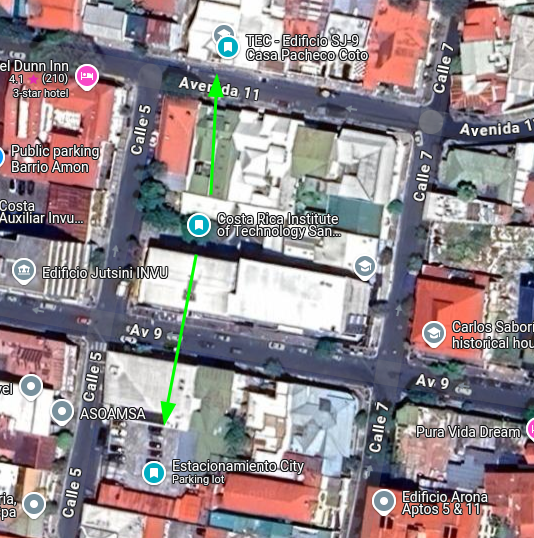
\includegraphics[width=0.8\textwidth]{fig/proy/ubiacion_parqueos.png}
	\caption{Ubicación de los parqueos obtenida mediante Google Maps.}
	\label{fig:ubiacion_parqueos}
\end{figure}

La entrada al estacionamiento interno se encuentra en el extremo opuesto de la entrada principal,
donde se encuentra ubicada la caseta del guarda de seguridad.
Para ingresar, los conductores deben primero detenerse frente a la caseta, notificar al guarda de seguridad
y luego rodear la cuadra hasta llegar al portón de acceso al parqueo.

Si no hay espacio disponible, se permite utilizar el estacionamiento de Casa Pacheco.
En ese caso, es necesario consultar con un guarda ubicado dentro del edificio si hay cupo.
Si la respuesta es afirmativa, el guarda de seguridad abre el portón manualmente para permitir
el ingreso del vehículo. Dado lo reducido del espacio, en algunas ocasiones el guarda debe asistir
a los conductores para maniobrar y estacionar adecuadamente.


Como última opción está el estacionamiento City. En cuanto a este estacionamiento,
también es necesario preguntar al personal de seguridad si hay espacios disponibles.
Si los hay, se abre el portón para que los vehículos puedan ingresar.


Cabe señalar que solo el portón del estacionamiento interno cuenta con un semáforo que indica si hay espacios disponibles.
Este semáforo es operado manualmente por los guardas de seguridad.

\begin{figure}[H]
	\centering
	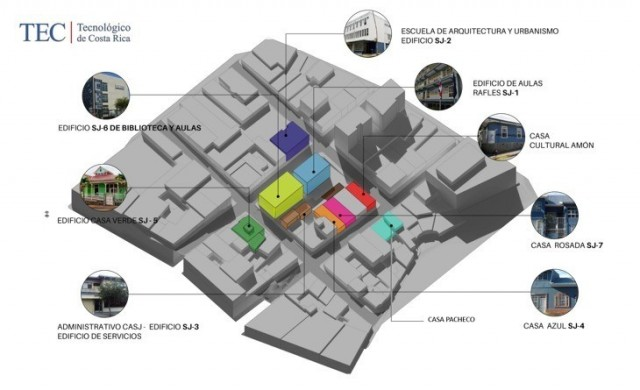
\includegraphics[width=0.8\textwidth]{fig/proy/croquis_del_campus_tec_san_jose.jpeg}
	\caption{Croquis del Campus Tecnológico Local San José \cite{tecCroquisSJ}.}
	\label{fig:croquis_tec}
\end{figure}

Actualmente, no existe una coordinación entre los distintos guardas para la gestión conjunta de los estacionamientos.
Además, las cámaras de seguridad instaladas en cada parqueo no pueden ser observadas por estos guardas,
ya que el monitoreo está a cargo de un grupo distinto ubicado en Casa Rosada,
dentro del campus principal (ver Figura \ref{fig:croquis_tec}).
Dicho grupo y los guardas de los parqueos operan de forma independiente, pues pertenecen a contratos diferentes.

El equipo de monitoreo en Casa Rosada tiene como responsabilidad principal la seguridad general del campus,
incluyendo la vigilancia ante robos y daños a la propiedad. Por su parte,
los guardas de los estacionamientos se encargan principalmente de controlar el ingreso de personas y vehículos.
Las horas de mayor uso del parqueo ocurren en las mañanas, entre las 7:00 a.m. y las 9:20 a.m.,
cuando se genera una leve congestión debido a la búsqueda de espacios disponibles.

\subsection{Reglamentos y logística}
Los automóviles que ingresan deben respetar un reglamento 
interno para garantizar la seguridad y el orden dentro del Campus.
Para tal propósito, al ingresar a la institución se debe registrar el número de placa y el nombre del usuario.
Adicionalmente, es aconsejable que los usuarios que ingresan estacionen sus vehículos
en lugares que no dificulten el ingreso o salida de nuevos vehículos cortando la visibilidad;
y así agilizar la movilidad dentro de estacionamiento y la búsqueda de estacionamiento.
En horas de alto flujo vehicular el registro y control de los vehículos que ingresan
genera cuellos de botella en la entrada del Campus, ralentizado el acceso y causando congestión.

\subsection{Factores tecnológicos}
En cada uno de los estacionamientos existe una cámara de seguridad. En el estacionamiento interno,
esta cámara está observando la entrada principal en una vista elevada, y también tiene una vista elevada del estacionamiento. 
En Casa Pacheco hay una única cámara que solo apunta a la entrada. Está en una pared al fondo y permite 
observar parcialmente la ubicación de los automóviles según lo reportado por el equipo de monitoreo.
Sin embargo, esta cámara por el momento está inactiva a espera de mantenimiento.
En el estacionamiento City hay un cámara con vista elevada desde la esquina suroeste. Da una vista desde arriba de todos
los automóviles en el estacionamiento. La institución solo tiene acceso a la
cámara del estacionamiento interno. A las cámaras de Casa Pacheco y Estacionamiento City solo tiene acceso 
monitoreo en Casa Rosada. Los guardas de seguridad de cada estacionamiento no tienen acceso a ninguna de las cámaras.

\section{Experiencias previas de control vehicular en el TEC}
En un primer intento por abordar la problemática de gestión vehicular,
el Campus Tecnológico Local San Carlos solicitó la implementación de un sistema de reconocimiento automático
de placas vehiculares (ANPR) como parte de un sistema más amplio de gestión inteligente de parqueos (IPLMS).
Este proyecto inicial buscaba aprovechar los recursos ya existentes en dicha sede, como las cámaras de seguridad,
con el objetivo de mejorar la coordinación y uso eficiente de los espacios de estacionamiento.

El diseño original logró realizar parcialmente la identificación de las placas,
pero no alcanzó un reconocimiento óptimo de los caracteres alfanuméricos.
En pruebas realizadas, se obtuvo una tasa de éxito aceptable (91\%) para placas de otros países,
pero esta se redujo drásticamente a un 40\% en el caso de placas costarricenses,
debido principalmente a la falta de datos representativos en el proceso de entrenamiento del sistema \cite{proyecto_previo}.

Posteriormente, el Campus Tecnológico Local San José mostró interés en el proyecto.
Dado que esta sede se encuentra más cerca del Campus Central en Cartago —donde se ubica el equipo desarrollador—, 
resultó más conveniente llevar a cabo pruebas y mejoras en San José.
Por este motivo, el presente proyecto se enfoca en resolver la problemática de dicha sede,
aunque se plantea desde su concepción una solución adaptable,
de modo que en el futuro pueda ser implementado también en la sede de San Carlos.

El sistema desarrollado anteriormente se apoyó en redes neuronales convolucionales (CNN)
y bibliotecas de código abierto como YOLO (You Only Look Once). Sin embargo,
no se tomaron en cuenta diferencias importantes entre las condiciones ambientales de San Carlos y San José.
Por ejemplo, en el Campus San Carlos las cámaras estaban ubicadas en ángulos favorables y
existían barreras vehiculares (agujas) que permitían al sistema capturar imágenes con suficiente tiempo
para hacer la lectura de placas, como se observa en la Figura~\ref{fig:anpr san carlos camara}.

\begin{figure}[H]
	\centering
	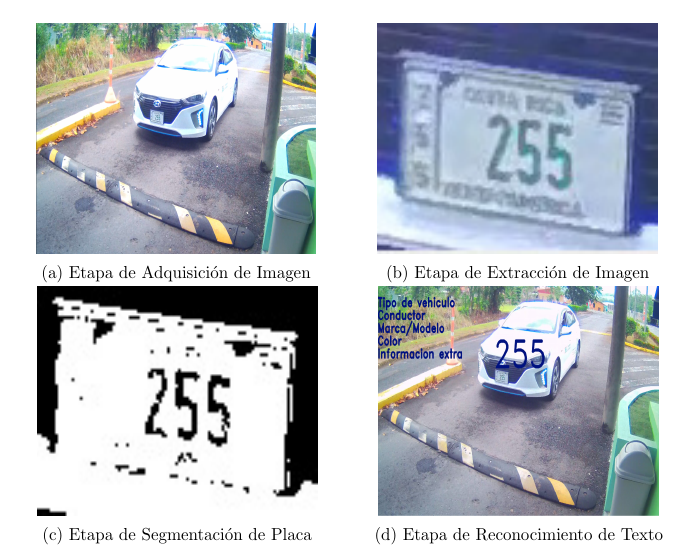
\includegraphics[width=0.8\linewidth]{fig/proy/ANPR_san_carlos.png}
	\caption{Etapas del ANPR.}
	\label{fig:anpr san carlos camara}
\end{figure}

Por el contrario, en la sede de San José, los vehículos ingresan rápidamente y no hay barreras que los detengan,
lo que reduce el tiempo disponible para la captura de imágenes. Además,
aunque se intentó reutilizar las cámaras existentes, estas no pueden ser reubicadas por motivos de seguridad.
Su ubicación actual--—en puntos elevados y con ángulos inclinados—--,
junto con condiciones de iluminación adversas (sol directo en las mañanas y escasa luz en las noches),
dificulta la visibilidad y complica el funcionamiento del sistema ANPR.
Aunque se usaron imágenes de placas costarricenses durante el entrenamiento,
estas fueron tomadas mayoritariamente en condiciones ideales: de día y en ángulos frontales,
lo que introdujo un sesgo en los datos.

Por estos motivos, el proyecto anterior no se llegó a implementar en ninguna de las dos sedes 
y actualmente se encuentra suspendido.

Dado que no se dispone de imágenes oficiales de las cámaras de seguridad ni de los equipos instalados
---por razones de seguridad institucional---, se ha optado por utilizar un croquis representativo para ilustrar 
la distribución aproximada de estos elementos dentro del campus. Esta representación no pretende ser un plano técnico,
sino una herramienta visual de apoyo que permite comprender mejor el contexto operativo 
en el que se desarrollará la solución propuesta.

\begin{figure}[H]
    \centering
    % Fila pacheco
    \begin{subfigure}[t]{0.45\textwidth}
        \centering
		\placeholderimage{0.3\textwidth}
        % \includegraphics[width=\linewidth]{fig/proy/example-image-pacheco_croquis_front}
        \caption*{Pacheco - Vista frontal}
    \end{subfigure}
    \hfill
    \begin{subfigure}[t]{0.45\textwidth}
        \centering
		\placeholderimage{0.3\textwidth}
        % \includegraphics[draft,width=\linewidth]{fig/proy/example-image-pacheco_croquis_up}
        \caption*{Pacheco - Vista superior}
    \end{subfigure}
    
	\vspace{1em}
	
	%Fila city
    \begin{subfigure}[t]{0.45\textwidth}
        \centering
		\placeholderimage{0.3\textwidth}
        % \includegraphics[draft,width=\linewidth]{fig/proy/example-image-city_croquis_front}
        \caption*{City - Vista frontal}
    \end{subfigure}
	\hfill
    \begin{subfigure}[t]{0.45\textwidth}
        \centering
		\placeholderimage{0.3\textwidth}
        % \includegraphics[draft,width=\linewidth]{fig/proy/example-image-city_croquis_up}
        \caption*{City - Vista superior}
    \end{subfigure}
	
	\vspace{1em}

    % Fila principal
    \begin{subfigure}[t]{0.45\textwidth}
        \centering
		\placeholderimage{0.3\textwidth}
        % \includegraphics[draft,width=\linewidth]{fig/proy/principal_croquis_front.png}
        \caption*{Principal - Vista frontal}
    \end{subfigure}
	\hfill
    \begin{subfigure}[t]{0.45\textwidth}
        \centering
		\placeholderimage{0.3\textwidth}
        % \includegraphics[draft,width=\linewidth]{fig/proy/principal_croquis_up.png}
        \caption*{Principal- Vista superior}
    \end{subfigure}
    \caption{Croquis de los sitios evaluados: Casa Pacheco, Estacionamiento City y Estacionamiento Principal.}
\end{figure}

\section{Retos en el control de acceso y disponibilidad de parqueos en el Campus San José}

El problema a solucionar es que el Campus Tecnológico Local San José del TEC presenta dificultades
para encontrar y acceder a espacios de estacionamiento, debido a la falta de coordinación entre
los distintos estacionamientos, la escasa visibilidad sobre su disponibilidad y la dependencia
de procedimientos manuales, lo que provoca molestias y pérdida de tiempo.

\section{Propuesta de un sistema de detección y reconocimiento de placas vehiculares}

En el Campus Tecnológico Local San José existen dificultades para encontrar
lugar de estacionamiento. Dada la descoordinación que existe entre los tres estacionamientos
de la universidad a los conductores se les dificulta encontrar con rapidez un lugar para estacionar.
Por ello se busca que las soluciones propuestas brinden al menos los siguientes requerimientos generales:

\begin{enumerate}
	\item Mejorar la gestión de espacios de estacionamiento en el Campus San José del TEC.
    \item Facilitar el acceso a información sobre disponibilidad de espacios.
	\item Usar recursos existentes cuando sea posible.
\end{enumerate}

Se espera entonces mejorar la fluidez de acceso a los estacionamientos brindando información a 
los conductores y guardas de seguridad para poder gestionar de forma más eficiente los estacionamientos,
facilitando encontrar lugar de estacionamiento y manteniendo orden en el lugar.
Asimismo, al aprovechar los recursos existentes, cámaras de video y computadoras, se puede brindar el 
prototipo de una solución de bajo costo para la institución.

En la propuesta de solución, que se brindará a continuación, se considerará la posibilidad de
extender la solución al Campus Tecnológico Local San Carlos.
Puesto que si bien el proyecto es solo para la Sede de San José, el Campus de San Carlos
ha manifestado el deseo de aplicar la solución también en dicha institución.

La propuesta en cuestión es el prototipo de un subsistema encargado de detección y 
reconocimiento de números de placas vehiculares (ANPR),
que será usado en un proyecto mayor de gestión inteligente de estacionamientos (IPLMS).
El sistema consta de cámaras instaladas en los accesos a los estacionamientos que envían los
datos capturados a un servidor local. Este servidor ejecutará un software IPLMS, que procesa la 
información en tiempo real. 
Los datos procesados son compartidos con dos salidas: una aplicación web,
donde los usuarios consultan la disponibilidad de espacios libres,
y un semáforo en la entrada de cada estacionamiento, que indica si existen espacios o no.

Dada la complejidad de un sistema completo de gestión de parqueos,
en este trabajo se aborda únicamente la etapa de reconocimiento automático de placas vehiculares (ANPR).
El subsistema ANPR consiste en aproximación mediante redes neuronales end-to-end. 

Los sistemas segmentados tradicionales presentan limitaciones:
dependen de conocer la cantidad de caracteres,
son sensibles a condiciones ambientales (iluminación, ángulo de visión, deformaciones),
y su desempeño está limitado por el “eslabón más débil” del pipeline, lo que dificulta su reajuste.

Una red end-to-end mitiga estos problemas al integrar todo el proceso de reconocimiento 
en una única arquitectura de aprendizaje profundo. Sin embargo, esto requiere grandes volúmenes 
de datos para entrenamiento \cite{endToEndDepthwise}. Para suplir esta carencia se desarrollará 
un generador de datos sintéticos de placas, que permita entrenar el modelo de reconocimiento de manera robusta.

La propuesta de solución se organiza en dos etapas principales: detección y reconocimiento, según los siguientes principios:

\begin{enumerate}

	\item \textbf{Captura de imágenes:}
Se emplean cámaras electrónicas instaladas en puntos estratégicos donde las placas sean visibles 
al ingreso de automóviles y motocicletas.


\item \textbf{Detección de placa:}  
      Se utiliza una red neuronal de detección de objetos para localizar y extraer la región correspondiente a la matrícula.  
      Existen múltiples modelos pre-entrenados que pueden adaptarse; en este caso se adopta **YOLOv11** 
		por su velocidad y precisión en tiempo real.  

\item \textbf{Reconocimiento de placa:}  
	A diferencia de los métodos basados en segmentación de caracteres, se emplea un modelo \textbf{end-to-end} 
		que integra la extracción y reconocimiento en una sola red convolucional.  
		Se consideran arquitecturas basadas en \textbf{CNN + CTC},
		entrenadas con datos sintéticos generados y posteriormente ajustadas con muestras reales.  

\end{enumerate}

\begin{figure}[H]
	\centering
	\placeholderimage{0.3\textwidth}
	% \includegraphics[width=\textwidth]{fig/proy/digrama-flujo-ANPR.jpg}
	\caption{Diagrama de flujo de sistema ANPR}
\end{figure}

\section{Objetivos del proyecto y organización del documento}

\textbf{Objetivo general: }

Desarrollar un prototipo de 
sistema automático para la detección y reconocimiento de caracteres en placas vehiculares costarricenses,
aplicando técnicas de visión por computadora y aprendizaje automático,
adaptado a las condiciones del Campus Local San José del Tecnológico de Costa Rica.

\textbf{Indicador:}
	\begin{enumerate}
		\item \textbf{Mejora relativa de desempeño frente al sistema base} \\
		\textbf{Descripción:} Comparación del desempeño general (en CAR, EMR, IoU) del sistema
		desarrollado frente a una solución base no entrenada localmente (ejemplo YOLOv8 + EasyOCR). \\
		\textbf{Unidad:} Porcentaje (\%) de mejora promedio en métricas clave. \\
		\textbf{Criterio de cumplimiento:} Mejora $\geq$ 5\%, con margen de tolerancia del $\pm 2$\% respecto a referencia. \\
		\textbf{Justificación:} Evalúa si el sistema propuesto aporta una mejora significativa frente
			solución genérica sin ajuste local. Al tratarse de un sistema orientado a condiciones específicas del campus,
			se espera una mejor de detección y reconocimiento. \\\\
	\end{enumerate}

\textbf{Objetivos específicos: }
\begin{enumerate}
	\item Preparar un conjunto de datos adecuado para el entrenamiento del sistema,
		combinando imágenes reales de placas vehiculares costarricenses con datos sintéticos generados por software.
		
		\textbf{Indicador}:
		\begin{enumerate}
			\item \textbf{Tamaño mínimo de dataset útil para entrenamiento}\\
			\textbf{Descripción:} Número de imágenes reales anotadas disponibles para entrenar el modelo \\
			\textbf{Unidad:} Imágenes \\
			\textbf{Criterio:} Se requiere obtener y etiquetar al menos 700 imágenes reales. \\
			\textbf{Criterio de cumplimiento:} Se cumple si el dataset base alcanza $\geq$ 700 imágenes reales etiquetadas. \\
			\textbf{Justificación:} Un volumen mínimo de datos reales es necesario para entrenar modelos
				de forma que aprenda característica de placas reales y no sobreajuste sobre datos sintéticos. \\ \\
		\end{enumerate}

		\textbf{Entregable}: Conjunto de datos etiquetado (mínimo 700 imágenes reales y datos sintéticos generados).

	\item Implementar técnicas de aumento de datos en tiempo real durante el entrenamiento para 
		robustecer el modelo ante condiciones adversas de iluminación, ángulo y resolución.

		\textbf{Indicadores:}
		\begin{enumerate}
			\item \textbf{Presencia de aumento de datos en el pipeline de entrenamiento} \\
			\textbf{Descripción:} 
			Verifica si se aplican transformaciones visuales en tiempo real en el conjunto de entrenamiento \\
			\textbf{Unidad:} Cumplimiento binario (Sí/No) \\
			\textbf{Criterio:}  El modelo aplica rotaciones, ruido, 
				distorsiones o transformaciones similares al menos en un 50\% de los datos. \\ 
			\textbf{Criterio de cumplimiento:} Si se verifica en código y entrenamiento que se aplican aumentos. \\
			\textbf{Justificación:} La aplicación de aumentos fortalece la capacidad del modelo
				para responder a variaciones reales en ángulo, iluminación y resolución,
				lo cual es especialmente importante en ambientes no controlados \\

			\item \textbf{Variación de desempeño con y sin aumento de datos} \\
			\textbf{Descripción: }Evalúa si el modelo entrenado con aumento presenta mayor robustez frente a perturbaciones \\
			\textbf{Unidad: }Diferencia porcentual de CAR / EMR \\
			\textbf{Criterio: }La caída de precisión ante perturbaciones debe ser menor 
			en el modelo con aumento que en uno sin aumento. \\
			\textbf{Criterio de cumplimiento:} Si $\Delta$ caída es menor o igual al $\leq$ 5\%
				frente a perturbaciones comparado con baseline sin aumento. \\
			\textbf{Justificación}:  Este indicador permite comprobar que los aumentos de datos no solo están presentes,
				sino que realmente aportan robustez y hacen al sistema menos sensible a perturbaciones\\ \\
		\end{enumerate}

		\textbf{Entregables}: Módulo o script configurado de aumento de datos integrado al pipeline de entrenamiento

	\item Diseñar y entrenar una arquitectura de reconocimiento automático de placas basada en una red neuronal convolucional 
		moderna (end-to-end), que incluya una etapa de detección de región de placa 
		y otra de reconocimiento de texto sin segmentación manual.

		\textbf{Indicador}:
		\begin{enumerate}
			\item \textbf{Tipo de arquitectura desarrollada} \\
			\textbf{Descripción: }Características que debe poseer la arquitectura diseñada de detección
				y reconocimiento de placa. \\
				\textbf{Unidad: }Binario (Si/No). \\
			\textbf{Criterio: }Arquitectura no segmentada + entrada imagen con salida texto. \\
			\textbf{Criterio de cumplimiento:} El sistema presenta bloques claramente identificados \\
				(detección, reconocimiento, entrada imagen y salida de texto). \\
			\textbf{Justificación:}  Asegura que el sistema sea moderno y capaz
				de reconocer placas completas sin necesidad de separar caracteres manualmente \\\\
		\end{enumerate}

		\textbf{Entregables:} Modelos entrenados y listos para inferencia (detección y reconocimiento).

	\item Evaluar el desempeño del sistema propuesto comparándolo contra un modelo base
		mediante métricas de reconocimiento y detección, con el fin de validar mejoras en precisión,
		exactitud completa y robustez.

		\begin{enumerate}
			\item \textbf{Tasa de reconocimiento de caracteres (Character Accuracy Rate, CAR)} \\
				\textbf{Descripción:} Mide la proporción de caracteres correctamente reconocidos por el modelo. \\
				\textbf{Unidad:} Porcentaje (\%) \\
				\textbf{Criterio de evaluación:} 
					Se considera aceptable si el modelo es mejora respecto de la línea base. \\
				\textbf{Criterio de cumplimiento:} Mejora$\geq 5\%$. \\
				\textbf{Justificación:}  El CAR mide la capacidad del sistema para reconocer caracteres individuales
				correctamente. Es una métrica central para evaluar la precisión del reconocimiento parcial de placas,
				especialmente útil cuando algunas predicciones son parcialmente correctas. \\
			\item \textbf{Error de secuencia completa (Exact Match Rate)} \\
				\textbf{Descripción:}
				Proporción de placas en las que se predice correctamente la secuencia completa de caracteres. \\
				\textbf{Unidad:} Porcentaje (\%) \\
				\textbf{Criterio:} Mejora la capacidad de reconocimiento total entre la secuencia predicha y la real. \\
				\textbf{Criterio de cumplimiento:} Mejora$\geq 10\%$ \\
				\textbf{Justificación:}  El EMR evalúa la proporción de placas completamente reconocidas sin errores.
				Esta métrica representa un caso ideal de éxito y es crítica para determinar si el sistema 
				puede ser usado en contextos donde los errores de una letra o número no son tolerables. \\
			\item mIoU (Mean Intersection over Union) en detección de placas \\
				\textbf{Descripción:} Evalúa qué tan bien se detecta la región de la placa en relación con la anotación real. \\
				\textbf{Unidad:} Valor entre 0 y 1 \\
				\textbf{Criterio:} Se considera aceptable si detecta mejor la placa respecto al modelo base. \\
				\textbf{Criterio de cumplimiento:} Mejora$\geq0.03$ \\
				\textbf{Justificación}:  mIoU mide qué tan bien el sistema detecta la región de la placa.
				Esta métrica es esencial para garantizar que el texto reconocido provenga de la región correcta
				de la imagen y no se contamine con información visual irrelevante.\\ \\
		\end{enumerate}

		\textbf{Entregables:} Documentación y reporte técnico de resultados de las evaluaciones.
\end{enumerate}

En cuanto a la estructura, este documento se organiza de la siguiente manera:
\begin{itemize}
    \item El \textbf{Capítulo 1} presenta la introducción, incluyendo el contexto, 
		antecedentes, el problema, un esbozo de la solución y los objetivos.
    \item El \textbf{Capítulo 2} expone el marco teórico y el estado del arte en sistemas
		de reconocimiento de placas y gestión de estacionamientos inteligentes.
    \item El \textbf{Capítulo 3} describe la metodología empleada para el desarrollo de la solución.
    \item El \textbf{Capítulo 4} detalla los resultados obtenidos y el análisis de desempeño del sistema.
    \item Finalmente, el \textbf{Capítulo 5} presenta las conclusiones y recomendaciones para trabajos futuros.
\end{itemize}


\section{Sistema de almacenamiento energético}

Después de las secciones anteriores ya ha guiado al lector hasta este
punto en donde solo resta presentar una propuesta general de solución
del problema técnico concreto.

Para aclarar la solución se hace uso de un diagrama de bloques (ver
\figref{fig:diagbloques}) o diagrama de flujo general, es decir,
desde un nivel de abstracción muy alto, donde no sea necesario entrar
en detalles técnicos, porque aún no han sido expuestos.


  \chapter{Marco teórico}
\label{ch:marco}

\section{Descripción}

Toda tesis hace referencia a trabajos previos en el área y trabajos afines que
están directamente relacionados con lo planteado en el tesis.

Además, en el marco teórico debe aparecer la información absolutamente
necesaria para comprender la solución, y por eso es recomendable escribir
primero la solución (el siguiente capítulo), para ir anotando qué debe ser
explicado en el marco teórico.

\section{Generalidades}

\begin{comment}
Se recomienda revisar las guías de publicación de la \nt{IEEE} en
\url{http://www.ieee.org/publications_standards/publications/authors/authors_journals.html},
donde puede encontrar cómo hacer referencias bibliográficas
correctamente, cómo citar ecuaciones, cuadros y figuras, etc.  Además,
puede buscar en Google por la última versión del ``Biblatex Cheat
Sheet'' para el resumen de cómo construir correctamente cada
referencia.

\end{comment}

\subsection{Redacción}

La \nt{redacción} en todo el documento debe seguir un estilo científico
objetivo. Esto implica que se redacta de modo impersonal, sin utilizar primeras
personas del singular o del plural, y se evita el uso de cualquier tipo de
calificativo, sustituyéndolos siempre por datos concretos, vinculados a
referencias bibliográficas o datos experimentales. Los comparativos también
deben concretarse a hechos y datos, y nunca dejarse ``en el aire''. Por la
naturaleza de la tesis, el tiempo verbal es usualmente presente, no perdiendo
nunca de vista que se está explicando ``cómo hacer algo'', en vez de ``qué se
hizo''.

Las \nt{frases} deben ser cortas, y debe evitarse que el lector tenga que saltar
constantemente entre partes de la tesis, lo que implica una exposición lineal
clara, donde lo que se necesita ya ha sido explicado antes. Deben evitarse
redundancias y por tanto cada concepto se exponen en un único lugar.

Todo aspecto circunstancial es irrelevante para la tesis, es decir, si se ha
desarrollado en el laboratorio $X$, o en el curso $Y$, con el profesor $Z$, o
en la empresa $W$, el nombre de funciones o clases en su código, etc., es
información irrelevante para reproducir el experimento, y por lo tanto sobra.
%
Esa información puede incluirse en uno de los anexos.

\begin{comment}
\subsubsection{Numeración del documento}

La primera página de la tesis es la correspondiente a la introducción,
así que ésta debe ser la página 1. Desde la introducción, hasta antes
de la bibliografía, las unidades son ``Capítulos''. La bibliografía y
anexos no se consideran capítulos, así que ya no continúan con la
misma numeración de los capítulos (la paginación sí continua). Los
índices, notación, glosario, etc.\ se numeran con números romanos en
versalitas ({\textsc{I}, \textsc{II}, \textsc{III}, \textsc{IV},
  \textsc{V}, \textsc{VI}}$\ldots$) y antes del índice (portada,
resúmenes, agradecimientos, hoja de evaluadores, etc.) las páginas no
llevan numeración.

Esta plantilla LaTeX ya se ocupa de todo lo anterior.

\subsection{Ecuaciones}

Para citar \nt{ecuaciones} se utilizan siempre paréntesis redondos, y
no es necesario emplear explícitamente la palabra ``ecuación''. Por
ejemplo ``Introduciendo en (4.2) los resultados de (3.3) y (3.7) se
obtiene ...''.  Se usa la palabra ``Ecuación'' solo si la frase inicia
con ello.  Por ejemplo ``La ecuación~\equ{eq:ej1} permite calcular la
corriente.''.

A diferencia de figura y cuadro, toda ecuación es parte del flujo de
texto y no un objeto flotante, así que \textbf{no} pueden emplearse de
la misma forma que las figuras o cuadros.  Esto es, cuando se requiere
introducir una ecuación, se pone directamente donde se necesita y por
tanto no es necesario citarla.

Es \textbf{incorrecto} redactar de la siguiente forma: \explain{MAL}

\textsl{La operación del transistor sin tomar en cuenta el efecto Early está
  dada por \equ{eq:ej1}, donde el parámetro $\kappa$ está dado por
  \equ{eq:ej2}.}

\begin{equation} \label{eq:ej1}
  I_{DS}
  =
  I_{n0} \frac{W}{L}e^{\kappa \frac{V_{GB}}{v_t}}
  \left[
    e^{-\frac{V_{SB}}{v_t}}
    -
    e^{-\frac{V_{DB}}{v_t}}
  \right]
\end{equation}

\begin{equation} \label{eq:ej2}
  \kappa = \frac{C_{ox}}{C_{ox}+C_{dep}}
\end{equation}

Lo anterior es incorrecto porque obliga al lector a estar buscando
ecuaciones, que pueden mostrarse directamente.  La única
referenciación de ecuaciones aceptable es hacia atrás.

La forma correcta de redactar lo anterior es: \chk{BIEN}

\textsl{La operación del transistor sin tomar en cuenta el efecto Early está
  dada por}
\begin{equation} \label{eq:ej3}
  I_{DS}
  =
  I_{n0} \frac{W}{L}e^{\kappa \frac{V_{GB}}{v_t}}
  \left[
    e^{-\frac{V_{SB}}{v_t}}
    -
    e^{-\frac{V_{DB}}{v_t}}
  \right]
\end{equation}
\textsl{donde el parámetro $\kappa$ es}
\begin{equation} \label{eq:ej4}
  \kappa = \frac{C_{ox}}{C_{ox}+C_{dep}}
\end{equation}

Esta plantilla define el comando \verb+\equ{label}+ que se encarga de
escribir el número de ecuación entre paréntesis, y de que los
paréntesis sean parte del hipervínculo (por ejemplo \equ{eq:ej3}).
%
Usted puede por supuesto hacer las referencias directamente con
\verb+(\ref{label})+, pero eso solo pondrá el hipervículo en el
número (por ejemplo (\ref{eq:ej4})).

Así el flujo del texto guía al lector por las ecuaciones sin mayor esfuerzo.

Es recomendable numerar \emph{todas} las ecuaciones, de modo que en la revisión
del documento, o en futuras referencias a su documento de tesis todas las
ecuaciones puedan ser citadas sin requerir describir textualmente a cuál
ecuación se está haciendo referencia.

Es preferible utilizar coma decimal en vez de punto decimal, debido a
que es el estándar internacional.  El Diccionario Panhispánico de
Dudas aclara que en la actualidad se acepta el punto como separador
decimal, pero eso no quiere decir que sea preferible.  Esta plantilla
ya incorpora el uso del paquete de \LaTeX\ \code{icomma}, que se
encarga de realizar el espaciado correcto de la coma.  Cuando utilice
coma como signo de puntuación, deje un espacio posterior, para
asegurarse de que \code{icomma} no lo tome como separador decimal.

\begin{equation}
  \label{eq:normrnd}
  h(x)=\norm{\rand()-0,5}^2_2
\end{equation}

\subsection{Figuras}

Esta plantilla define los comandos \verb+\figref+, \verb+\lafigref+,
\verb+\Figref+ y \verb+\Lafigref+.  Estos generan referencias a
figuras, pero incluyendo el artículo ``la'', y asegurándose de que la
palabra ``figura'' quede dentro de la referencia, y además de que el
número de figura nunca quede huérfano en la siguiente línea.  El texto
creado inicia con mayúscula, si la primera letra usada es mayúscula.
Por ejemplo: \verb+\figref{fig:figtemplate}+ produce
``\figref{fig:figtemplate}'', donde \verb+fig:figtemplate+ es la
etiquita usada; o \verb+\Lafigref{fig:figtemplate}+ genera
``\Lafigref{fig:figtemplate}''.  Nótese que cuando se usa
\verb+\ref{label}+, únicamente el número de la referencia queda dentro
del hipervínculo.

Para asegurar la calidad de la presentación de las imágenes y
gráficas, usted debe conocer el hecho de que para el almacenamiento de
imágenes existen dos tipos de formato: las imágenes raster y las
imágenes vectoriales.

\subsubsection{Imágenes raster}
\index{imagen!raster}
Las imágenes raster son representadas por una rejilla de píxeles, en donde cada
píxel tiene un valor que representa al nivel de gris o el color. La
discretización espacial es ineludible, y la única forma de obtener buena
calidad es empleando tamaños grandes de la imagen que conduzcan a resoluciones
de al menos 300 puntos por pulgada en la impresión, lo que conlleva a archivos
de documentos de varios megabytes. Dentro de los formatos para almacenar
imágenes raster existen algunos con pérdida (como el JPEG) que producen en
imágenes sintéticas, como diagramas, estructuras ruidosas que dan una
apariencia de baja calidad a las figuras. Otros formatos (como PNG, BMP, TIFF o
GIF) no tiene pérdidas de información, pero los algoritmos de compresión no
pueden reducir el tamaño de las imágenes con los mismos factores de reducción
que los formatos con pérdidas. Este tipo de formatos debe utilizarse únicamente
para fotografías o capturas de escenas reales con cámaras digitales.

\subsubsection{Imágenes vectoriales}

\index{imagen!vectorial} Las imágenes vectoriales \textbf{deben} ser
empleadas en todo tipo de diagrama. En ellas no se almacenan píxeles,
sino las estructuras geométricas que componen la figura como círculos
(representado por posicion de su centro y su radio), rectángulos
(representados por sus esquinas), líneas, texto, etc. La mayoría de
programas para elaborar este tipo de diagramas, como Inkscape, XFig,
OpenOffice.org Draw, MS Visio, Adobe Illustrator, etc. proveen varios
formatos vectoriales que pueden ser insertados tanto en LaTeX como en
OpenOffice.org Writer (o MS Word). Los formatos más empleados son los
llamados metafiles, que incluyen al WMF, EMF. En LaTeX se utiliza por
lo general EPS o PDF. Recientemente se ha incrementado el soporte al
formato SVG, pero la calidad de la conversión no es la mejor, y el
tiempo de conversión suele ser excesivo.  

No debe cometerse el error de generar una imagen vectorial a partir de una
imagen raster, pues una vez realizada la discretización espacial no es posible
reconstruir los elementos geométricos que componen la imagen. Por ello, no
tiene ningún sentido generar un archivo EPS o WMF a partir de una imagen ya
almacenada en BMP, JPG, o PNG, pues lo único que ocurrirá es que se inserta la
figura raster tal cual en la imagen vectorial, sin implicar ninguna ganancia en
la calidad.

Esta plantilla de LaTeX administra la generación de ciertas figuras
por usted.  Puede colocar en el directorio \texttt{fig/} archivos EPS,
JPG, PNG, TIKZ, SVG, o GP (de GNUPlot) y el Makefile se encarga de
hacer todas las conversiones necesarias y dejar las figuras en el
directorio correspondiente en formato PDF.  En las siguientes
subsecciones se describen dos casos adicionales que resultan útiles
para realizar figuras más complejas.

\subsubsection{Figuras tikz}
\index{tikz}

Esta plantilla compila archivos con código en Tikz para generar
figuras.
%
En realidad, lo único que hace el Makefile es compilar con
\code{pdflatex} cualquier archivo \texttt{fig/*.tikz} y dejar el
resultado en el directorio de figuras, aunque el concepto fue pensado
particularmente para generar imágenes vectoriales utilizando las
características de Tikz, biblioteca de LaTeX que es utilizada cada vez
más por su enorme flexibilidad.
%
\begin{figure}[htb]
  \centering
  \includegraphics{figtemplate}
  \caption[Ejemplo de figura con tikz]{Ejemplo realizado con
    \texttt{tikz}.  Usted encuentra la plantilla en el directorio de
    figuras bajo el nombre \texttt{fig/figtemplate.tikz}.}
  \label{fig:figtemplate}
\end{figure}

\Lafigref{fig:figtemplate} muestra un ejemplo que se puede utilizar como
plantilla para generar figuras \texttt{tikz}.  La plantilla la
encuentra en el directorio de figuras y se llama
\code{figtemplate.tikz}.  En Internet se encuentran cientos de figuras
de ejemplo para realizar este tipo de figuras.

En el código fuente de la introducción \code{intro.tex} encuentra en
el diagrama de bloques otro ejemplo de cómo incrustar la figura Tikz
directamente en el lugar, aunque se advierte que eso no es
recomendable porque aumenta el tiempo de compilación del documento.
Considere esto particularmente si utiliza plataformas como
\href{https://overleaf.com}{Overleaf}, que tiene un tiempo de
compilación limitado.


\subsubsection{Figuras ltxfig/psfrag}

\index{psfrag}\index{ltxfig}
Cuando en el subdirectorio \texttt{fig/} se encuentran dos archivos con el
mismo nombre pero extensiones \texttt{ltxfig} y \texttt{psfrag}, por ejemplo
\texttt{prueba.ltxfig} y \texttt{prueba.psfrag}, entonces el Makefile asume que
usted desea crear una figura a partir del archivo \texttt{prueba.ltxfig},
creado con el programa \texttt{XFig}, sustituyendo los textos ahí presentes con
texto formateado con LaTeX.

\Lafigref{fig:ltxfig} ha sido creada con este esquema.  Revise los
archivos correspondientes en el directorio de figuras
\texttt{fig/ltxfig\_prototipo.*} para más detalles sobre su uso.

\begin{figure}[htb]
  \centering
  \includegraphics[width=0.9\textwidth]{ltxfig_prototipo}
  \caption{Ejemplo de imagen ltxfig/psfrag}
  \label{fig:ltxfig}
\end{figure}

\subsubsection{Figuras pstricks}  

\index{pstricks} Los archivos con extensión \texttt{.pstricks} en el
directorio \texttt{fig} se utilizan para generar cualquier tipo de
imágenes según el código que se contenga.  Es un concepto más general
que el el utilizado con el \texttt{ltxfig} de la sección anterior.
\Lafigref{fig:pstricks} ha sido creada con este esquema.  Puede revisar
los archivos \texttt{prototipo\_gnuplot*} como un ejemplo de su uso,
en donde de un archivo gnuplot (\texttt{\_.gp}) se genera un archivo
\texttt{\_.eps}, el cual es incluido en el archivo \texttt{.pstricks}
sustituyendo cadenas de texto por código LaTeX.

\begin{figure}[htb]
  \centering
  \includegraphics{prototipo_gnuplot}
  \caption{Ejemplo de imagen gnuplot/pstricks}
  \label{fig:pstricks}
\end{figure}

\subsubsection{Subfiguras}

En la plantilla ya se incluye el paquete \code{subcaption}, que es el
sucesor del paquete \code{subfig} que a su vez es el sucesor de
\code{subfigure}.  Los dos paquetes anteriores tienen muchos problemas
con el paquete \code{hyperref} y por tanto es mejor evitarlos.
\Lafigref{fig:subfiguras} muestra un ejemplo con dos figuras, donde por
ejemplo, \lafigref{fig:subfigura_a} es un circuito.  La
documentación del paquete \code{subcaption} presenta abundancia de
casos con y sin leyendas en las subfiguras y cómo referenciarlas
correctamente.

\begin{figure}[htb]
  \centering
  \subcaptionbox{\label{fig:subfigura_a}}%
    {\includegraphics[scale=0.6]{figtemplate}}
  \subcaptionbox{\label{fig:subfigura_b}}%
    {\includegraphics[scale=0.6]{prototipo_gnuplot}}
  \caption[Ejemplo de figuras con subcaption]{Este es un ejemplo de
      uso de subfiguras con subcaption.  (a) Un circuito.  (b) Una
      función.}
  \label{fig:subfiguras}
\end{figure}


\subsubsection{Entradas en el índice de figuras}

El índice de figuras debe servir para encontrar rápidamente dónde se
encuentra cierta figura.  El pie de la figura, indicado en \LaTeX con
\verb+\caption+ puede ser extenso, en especial para indicar detalles
de las figura.  Lo indicado con \verb+\caption+ es la entrada que por
defecto aparecerá en el índice de figuras.  Sin embargo, en el índice
la referencia a cada figura no debe superar la extensión de una línea
y debe únicamente dar la idea del contenido de la figura, para que
pueda ser encontrada rápidamente.  Para lograr esto en \LaTeX{} se
agrega un parámetro opcional con el texto del índice, de la siguiente
forma:
\begin{verbatim}
  \caption[Texto en el índice]{Texto al pie de la figura}
\end{verbatim}
Esto funciona también con \lastablas.


\subsection{Cuadros o tablas}

¿Se dice tabla o cuadro? Esta es una pregunta no tan simple de
responder.  \LaTeX, o mejor dicho el paquete \code{babel} para
español, por defecto define a las leyendas (\verb+\caption+) del
entorno \verb+table+ como \emph{cuadro}.  Sin embargo, en
Latinoamérica, en particular por influencia del inglés, se ha
extendido la traducción de \emph{table} como \emph{tabla}.

Formalmente en español se debería diferenciar entre ambas: la tabla
usualmente contiene datos que se referencian directamente, como las
tablas de logaritmos, la tabla periódica de los elementos, las tablas
de multiplicar, las tablas de transformadas, etc.  Los resultados de
un análisis experimental se sintetizan en lo que en español se
denomina \emph{cuadros}, y puesto que la mayoría de tesis e informes
de proyecto lo que se usan son precisamente \emph{cuadros}, entonces
\LaTeX\ para español define por defecto ese término.

En esta plantilla está activo el uso de \emph{tabla}, por ser esta la
tradición en la Escuela de Ingeniería Electrónica, pero basta eliminar
la opción \verb+es-tabla+ en el paquete \verb+babel+ en
\code{macros.tex} para reactivar el uso por defecto de \emph{cuadro}.

Si usted no tiene aún claro si desea usar \emph{cuadro} o
\emph{tabla}, utilice los comandos listados en
\latabref{tab:comandostab}, y así todo cambiará automáticamente de
acuerdo a la opción que se especifique para babel.  La tercera columna
muestra la salida de los comandos en la actual compilación del
documento.  Usted puede cambiar la opción de \verb+babel+ en
\code{macros.tex} y observar el cambio.

%\afterpage{% Esto es para forzar que la tabla salga después de la
%           % figura grande
\begin{table}[htb]
  \centering
  \caption[Comandos para cuadro o tabla]{Comandos definidos para
    cambiar cuadro o tabla según se indique al paquete babel.}
  \label{tab:comandostab}
  \begin{tabular}{llll}
    \toprule
    Comando & Con \verb+es-tabla+ & Sin \verb+es-tabla+ & Actualmente \\
    \midrule
    \verb+\cuadro+     & tabla      & cuadro      & \cuadro \\  
    \verb+\Cuadro+     & Tabla      & Cuadro      & \Cuadro \\  
    \verb+\elcuadro+   & la tabla   & el cuadro   & \elcuadro \\  
    \verb+\Elcuadro+   & La tabla   & El cuadro   & \Elcuadro \\  
    \verb+\loscuadros+ & las tablas & los cuadros & \loscuadros \\
    \verb+\Loscuadros+ & Las tablas & Los cuadros & \Loscuadros \\
    \verb+\tabla+      & tabla      & cuadro      & \tabla \\  
    \verb+\Tabla+      & Tabla      & Cuadro      & \Tabla \\  
    \verb+\latabla+    & la tabla   & el cuadro   & \latabla \\  
    \verb+\Latabla+    & La tabla   & El cuadro   & \Latabla \\  
    \verb+\lastablas+  & las tablas & los cuadros & \lastablas \\
    \verb+\Lastablas+  & Las tablas & Los cuadros & \Lastablas \\   
    \verb+\tabref{label}+
                       & tabla\verb+~\ref{label}+
                       & cuadro\verb+~\ref{label}+
                       & \tabref{tab:comandostab} \\
    \verb+\Tabref{label}+
                       & Tabla\verb+~\ref{label}+
                       & Cuadro\verb+~\ref{label}+
                       & \Tabref{tab:comandostab} \\
    \verb+\latabref{label}+
                       & la tabla\verb+~\ref{label}+
                       & el cuadro\verb+~\ref{label}+
                       & \latabref{tab:comandostab} \\
    \verb+\Latabref{label}+
                       & La tabla\verb+~\ref{label}+
                       & El cuadro\verb+~\ref{label}+
                       & \Latabref{tab:comandostab} \\
    \bottomrule
  \end{tabular}
\end{table}
%}

Observe que el comando \verb+\tabref+ se encarga de que la palabra
\emph{\tabla} quede como parte del enlace, mientras que si usted usa
directamente \verb+\ref+ entonces únicamente el número quedará
enlazado.

\subsubsection{Figuras enormes de una página en horizontal}

En ocasiones, es necesario colocar una figura o \tabla\ grande que no
cabe en el formato vertical de página.  Para esto, el entorno
\verb+sidewaysfigure+ permite rotar el contenido, aunque esto deja la
página en el archivo PDF generado en posición vertical, de modo que
cuando se lea por medios electrónicos, será incómodo interpretarlo, a
menos que activamente se rote todo el documento.  Una mejor opción es
entonces indicar directamente en el archivo PDF que se presente una
página en particular de forma horizontal, como lo ilustra la
\figref{fig:large}.
\afterpage{%
\clearpage
\begin{rotatepage}
\begin{sidewaysfigure}
  \centering
  \includegraphics[width=\textheight]{ltxfig_prototipo}
  \caption{Ejemplo de figura enorme.}
  \label{fig:large}
\end{sidewaysfigure}
\end{rotatepage}
}
\clearpage %% Necesario aquí porque el verbatim que sigue confunde a latex



Para eso se ha definido en la plantilla un entorno sencillo denominado
\verb+rotatepage+.  Se usa de la siguiente forma:
%
\begin{verbatim}
\afterpage{%
  \clearpage
  \begin{rotatepage}
    \begin{sidewaysfigure}
      \centering
      \includegraphics[width=\textheight]{ltxfig_prototipo}
      \caption{Ejemplo de figura enorme.}
    \end{sidewaysfigure}
  \end{rotatepage}
}
\end{verbatim}
%
El comando \verb+\afterpage+ da la instrucción de ejecutar el código
indicado justo después de terminar la página actual, en donde se
ordena primero pasar la página y sacar todos los objetos flotantes que
hayan quedado pendientes.  Esto tendrá el efecto secundarios de que si
en el resto de la página donde se coloca la inclusión de la figura hay
otros objetos flotantes, estos se colocarían primero.
%
Por ello, puede ser necesario que usted tenga que manipular esos
objetos flotantes para que aparezcan en otros lugares.

Siguiendo con el código de ejemplo, el entorno \verb+rotatepage+
intenta colocar los comandos de PDF necesarios para rotar la página.
Su implementación es muy sencilla y puede fallar.  Puede revisar su
implementación en el archivo {macros.tex}.



\subsection{Código}

Si usted necesita poner un ejemplo de código de descripción de
hardware o de algún lenguaje de programación, evite usar
``pantallazos'' pues al ser imágenes raster tiene baja calidad.

Puede insertar al código como figuras.  Si por la naturaleza del tema
de su proyecto o tesis hay más de diez ejemplos de código, quizá deba
buscar cómo agregar un nuevo tipo de objetos flotantes.

Se recomienda el uso del paquete \verb+listings+.  La plantilla define
en el archivo \code{macros.tex} un entorno para verilog, como se ilustra en la \figref{fig:verilog}.

\begin{figure}[htb]
  \begin{lstlisting}[style={verilog-style}]
    //-----------------------------------------------------
    // Design Name : mux_using_case
    // File Name   : mux_using_case.sv
    // Function    : 2:1 Mux using Case
    //-----------------------------------------------------
    module  mux_using_case(
      input  wire  din_0         , // Mux first input
      input  wire  din_1         , // Mux Second input
      input  wire  sel           , // Select input
      output reg [1:0]  mux_out    // Mux output (BUG IN HERE)
    );
    //-------------Code Starts Here---------
    always @ (*)
    MUX : begin
      case (sel) 
        1'b0 : mux_out = din_0;
        1'b1 : mux_out = din_1;
      endcase 
    end 
    
    endmodule //End Of Module mux
  \end{lstlisting}
  \caption[Ejemplo de código con listings.]{Ejemplo de uso de \code{listings}
    para insertar código Verilog, pero puede usarse para otros
    lenguajes.}
  \label{fig:verilog}
\end{figure}

\subsection{Referencias bibliográficas}

\index{referencias}\index{BibTeX} Todo concepto o idea tomado de otros
autores contar con la respectiva referencia. En redacción técnica de
ingeniería rara vez se utiliza la cita textual, así que es necesario
reformular las ideas y conceptos con palabras propias. En ingeniería
electrónica se utilizan los formatos de referencia de la IEEE o la
ACM, que son numéricos, encerrados entre paréntesis cuadrados (por
ejemplo, ``En \cite{Davis1963} se propuso un nuevo algoritmo'', o ``En
\cite{ProakisManolakis1998} los autores proponen tomar las ventajas de
los algorimos presentados
en~\cite{Oppenheim1998,Roberts2005,Haykin2001} por medio del método de
Newton \cite{Burrus1998} conocido en el área de optimización
lineal.''). La referencia es parte de las frases, así que si la frase
termina con la referencia para indicar la idea, ésta debe estar antes
del punto final o demás signos de puntuación: ``La capacidad de
memoria también sigue una Ley similar a la de Moore \cite{Octave}. Los
siguientes son los aspectos a tomar en cuenta en el diseño del sistema
\cite{Lindner2002}:''.  Las referencias múltiples usan un solo comando
\verb|\cite{Sorial2003,Shilov1973}|~\cite{Soria2003,Shilov1973}.

Se recomienda utilizar BibLaTeX para indicar las referencias
bibliográficas.  Actualmente herramientas como Mendeley, Zotero u
otras similares simplifican la administración de las referencias y
pueden exportar al formato BibTeX.

Si usa estos formatos, recuerde en los autores con dos apellidos
siempre usar
\begin{center}
  \code{author=\{apellidos, nombres and apellidos, nombres\}}  
\end{center}
o de lo contrario la generación de las referencias será incorrecta.

\subsection{Extensión}

\index{extensión}
Una tesis de licenciatura no debe sobrepasar las 120 páginas incluyendo
apéndices y los formalismos desde portada hasta índices.

El cuerpo de la tesis (desde introducción hasta conclusiones) usualmente se
extiende desde 45 páginas hasta no más de 80, dependiendo de la problemática
tratada.

No es necesario reproducir contenidos de otras fuentes: agregue las referencias
a dichas fuentes, y limítese a enunciar lo estrictamente necesario para
comprender sus propuestas de solución.

Contenidos que se salen de la línea principal de la tesis se colocan
en apédices, a los que se hace breve referencia (ver
apéndice~\ref{apx:apendice}).

\section{Sobre esta plantilla \LaTeX}

Esta plantilla \LaTeX pretende simplificar varios pasos en la creación
del documento de tesis.  Toda la configuración, incluyendo su nombre,
su número de carné, el nombre abreviado, el título del documento, la
fecha de defensa, el nombre de su asesor y sus lectores, etc.\ se
especifica en el archivo \code{config.tex}.

\subsection{Marcar asuntos pendientes}

La plantilla tiene dos ``\emph{modos}'' de operación: normal y
borrador (\emph{draft}).  En el archivo \texttt{config.tex}, en las
líneas 12 y 13 usted encuentra el código

\begin{verbatim}
\setboolean{draftmode}{true}            % turn draft mode on
%\setboolean{draftmode}{false}          % turn draft mode off
\end{verbatim}

Con el modo borrador, se activan ciertos comandos y funcionalidades
útiles en el proceso de elaboración de la tesis, pero que deben ser
desactivados al final, antes de entregar la tesis.  Por ejemplo, se
activa el pie de página que dice ``\emph{Borrador: fecha}'', y se
activa el índice titulado ``Revisar''.  En dicho índice aparecen las
páginas en donde se hayan utilizado alguno de los siguientes comandos:
\begin{compactitem}
\item \verb+\boxcomment{comentario}+ Crea una caja en el margen de página con
  el comentario indicado.
\item \verb+\explain{comentario}+ Crea una caja en el margen de página con
  el comentario indicado, con una flecha hacia la derecha para indicar qué en
  concreto debe ser revisado.
\item \verb+\chk{comentario}+ Crea una caja en el margen con símbolo de
  ``chequeado'' y el comentario indicado.
\item \verb+\TODO{comentario}+ Crea una caja grande de fondo sombreado con el
  comentario indicado.
\end{compactitem}

En este párrafo se\chk{resultado de chk} utilizan algunos de estos comandos
para ilustrar su efecto.  El \verb+\chk+ como puede observar tiene sentido
usarlo para marcar que algo está casi listo.  Por otro lado \explain{explain}
el comando \verb+\explain+ permite marcar algo que requiere ser revisado en
redacción, valores, etc.  El \verb+\boxcomment+\boxcomment{La caja simple}
solo pone una marca al margen.

\TODO{Finalmente el comando \texttt{TODO} coloca esta caja gris.}

Si usted desativa el modo draft, desaparecen todas las marcas
anteriores, y desaparece el índice ``Revisar''.  En éste índice
aparecen todas las páginas en donde se utilizaron estos comandos con
los respectivos comentarios, lo que permite encontrar rápidamente
detalles que usted indicó que debe revisar.

\subsection{Índices}

Como índice se conoce la lista de términos claves con su respectiva
página.  Usualmente aparece al final del documento.  La plantilla
ofrece varios comandos para simplificar el uso estandar del comando de
\LaTeX\ \verb+\index{término}+ que coloca al término indicado en el
índice.  Con \verb+\nt[indice]{término}+ (\emph{new term}) usted
indica la entrada principal del término, que aparece en el texto en el
índice, es decir, en el índice aparece lo que indique en vez de
``indice'' y en el texto aparece lo que indique ``término'';
\verb+\ot{término}+ agrega una entrada secundaria al término.

\end{comment}

  \chapter{Implementación del sistema de detección y reconocimiento de placas}
\label{ch:solucion}

\section{Generación sintética de imágenes}

La red neuronal end-to-end tiene la desventaja de requerir grandes cantidades de datos
para conseguir resultados con bajo error de entrenamiento y generalización;
habitualmente en el rango de 10 mil - 50 mil fotografías. 
En el tiempo disponible para la ejecución del proyecto no es posible 
capturar y etiquetar tal cantidad, además el costo de etiqueta de datos es 
elevado. El problema se mitiga utilizando imágenes sintéticas;
incrementando el conjunto de datos disponibles. 
Tales imágenes son creadas con base a la caracterización de las placas reales
y la fuente tipográfica usada en las mismas.

El conjunto artificial es utilizado para entrenar el modelo,
mientras que el conjunto de placas auténticas es usado
para la evaluación del sistema. Con ello se puede evaluar, indirectamente,
la utilidad de la estrategia, y la representatividad con la que conjunto sintético
asemeja al conjunto real en sus características esenciales.

En Costa Rica a las placas vehiculares se les asigna un código según el tipo de vehículos.
El reglamento sobre placas vehiculares especifica los códigos existentes, así como el color
del fondo de la placa y el color de los caracteres \cite{art97placasvehiculares}. Hay
más de 100 tipos de placas distintas.
Automóviles con códigos atípicos como el de placas extranjeras son poco probables de ser evaluadas;
además en el conjunto de imágenes reales no hay muestras de todos los tipos de placas.
Por este motivo solo se sintetizan placas basadas en las existentes en el conjunto de datos real
y las demás se dejan como casos no cubiertos o casos extremos. Los casos a cubrir se
muestran en la tabla \ref{tab:combinaciones-placas},
y sus características en \ref{tab:caracteristicas-placas}.

\begin{table}[H]
	\centering
	\begin{tabular}{|c|c|}
		\hline
			Tipo & Combinación \\
		\hline
			Particular & NNNNNN \\
		\hline
			Particular & LLL-NNN \\
		\hline
			TEC & 256 | NN \\
		\hline
			TEC & 256 | NNN \\
		\hline
			Carga ligera & CL | NNNNNN \\
		\hline
			Discapacitado & D-NNN \\
		\hline
			Motocicleta & M NNNNNN \\
		\hline
			Motocicleta & M $\frac{\text{NNN}}{\text{NNN}}$ \\
		\hline
	\end{tabular}
	\caption{Posible combinaciones de caracteres en placas costarricenses.}
	\label{tab:combinaciones-placas}
\end{table}

\begin{table}[H]
	\centering
	\begin{tabular}{|c|c|c|}
		\hline
			Código & Color placas & Color caracteres \\
		\hline
			 & Blanco & Azul \\
		\hline
			256 & Blanco & Verde \\
		\hline
			CL & Blanco & Rojo \\
		\hline
			 D & Blanco & Azul \\
		\hline
			 M & Blanco & Azul \\
		\hline
	\end{tabular}
	\caption{Características de placas costarricenses.}
	\label{tab:caracteristicas-placas}
\end{table}

Se producen los datos utilizando plantillas de placas reales y la fuente tipográfica real,
realizando recortes de los caracteres y dejando plantillas lo más limpias posibles.
Por ejemplo, las mostradas en Fig. \ref{fig:caracteres-full-azul} y \ref{fig:plantillas-full-blanco}.
Mediante software se crean placas aleatorias de forma sistemática,
tal como indica el diagrama de flujo \ref{fig:diagrama-flujo-generacion-multiples-placas}
y \ref{fig:diagrama-flujo-generador-placas}. 

\begin{figure}[H]
	\centering
	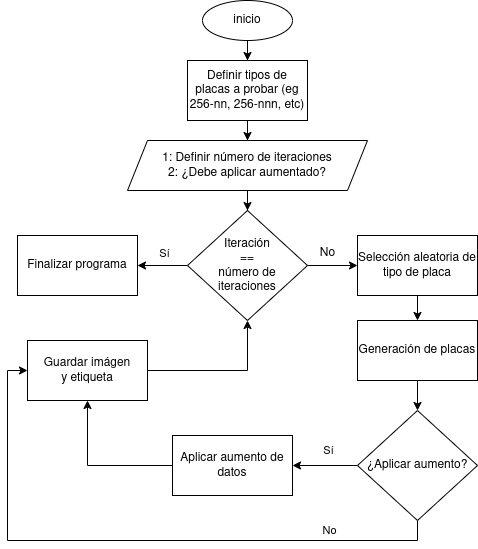
\includegraphics[width=\textwidth]{fig/proy/generacion-de-multiples-imagenes.drawio.png}
	\caption{Generación de múltiples imágenes sintéticas}
	\label{fig:diagrama-flujo-generacion-multiples-placas}
\end{figure}

\begin{figure}[H]
	\centering
	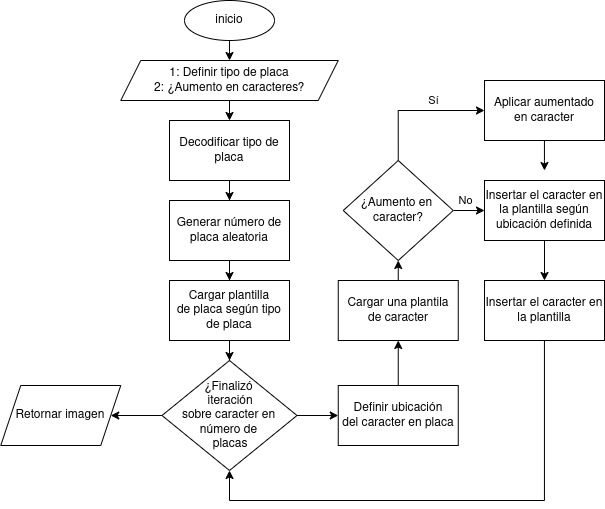
\includegraphics[width=\textwidth]{fig/proy/generacion-de-imagen-sintetica.drawio.png}
	\caption{Generación de imagen de placa sintética}
	\label{fig:diagrama-flujo-generador-placas}
\end{figure}

\section{Detección y extracción de ubicación de la placa en video e imágenes}

La detección de placas vehiculares en imágenes y video se realiza aplicando ajuste fino 
a modelos existentes. Se utiliza YOLOv11n.pt como principal, pues esta versión es 
más rápida y ofrece mejor capacidad de detección que sus predecesores. 
Se realiza además comparación de métricas con otras versiones de YOLO 
y con el modelo usado en el primer prototipo presentado en \cite{proyecto_previo}.

\section{Reconocimiento de número de placa}


  \chapter{Resultados y análisis}

\section{Características de las placas sintéticas generadas}
Algunos ejemplos de placas generadas son mostradas en Fig. \ref{fig:ejemplo-placas-sinteticas}

\begin{figure}[H]
    \centering
    % Fila pacheco
    \begin{subfigure}[t]{0.45\textwidth}
        \centering
        
\includegraphics[width=\linewidth]{fig/proy/synthetic_plate_1.png}
        % \caption*{Pacheco - Vista frontal}
    \end{subfigure}
    \hfill
    \begin{subfigure}[t]{0.45\textwidth}
        \centering
        
\includegraphics[width=\linewidth]{fig/proy/synthetic_plate_2.png}
        % \caption*{Pacheco - Vista superior}
    \end{subfigure}
    
	\vspace{1em}
	
	%Fila city
    \begin{subfigure}[t]{0.45\textwidth}
        \centering
        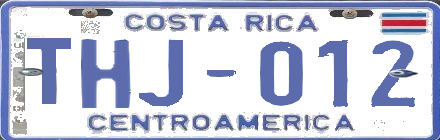
\includegraphics[width=\linewidth]{fig/proy/synthetic_plate_3.png}
        % \caption*{City - Vista frontal}
    \end{subfigure}
	\hfill
    \begin{subfigure}[t]{0.45\textwidth}
        \centering
        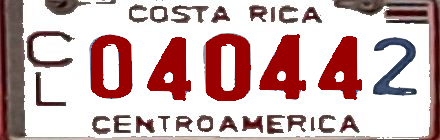
\includegraphics[width=\linewidth]{fig/proy/synthetic_plate_4.png}
        % \caption*{City - Vista superior}
    \end{subfigure}
	
	\vspace{1em}

    % Fila principal
    \begin{subfigure}[t]{0.45\textwidth}
        \centering
        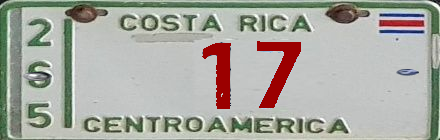
\includegraphics[width=\linewidth]{fig/proy/synthetic_plate_5.png}
        % \caption*{Principal - Vista frontal}
    \end{subfigure}
	\hfill
    \begin{subfigure}[t]{0.45\textwidth}
        \centering
        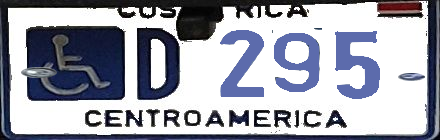
\includegraphics[width=\linewidth]{fig/proy/synthetic_plate_6.png}
        % \caption*{Principal- Vista superior}
    \end{subfigure}
    \caption{Ejemplos de placas sintéticas}
	\label{fig:ejemplo-placas-sinteticas}
\end{figure}

\section{Comparación de desempeño de detección de placas}

\begin{figure}[H]
	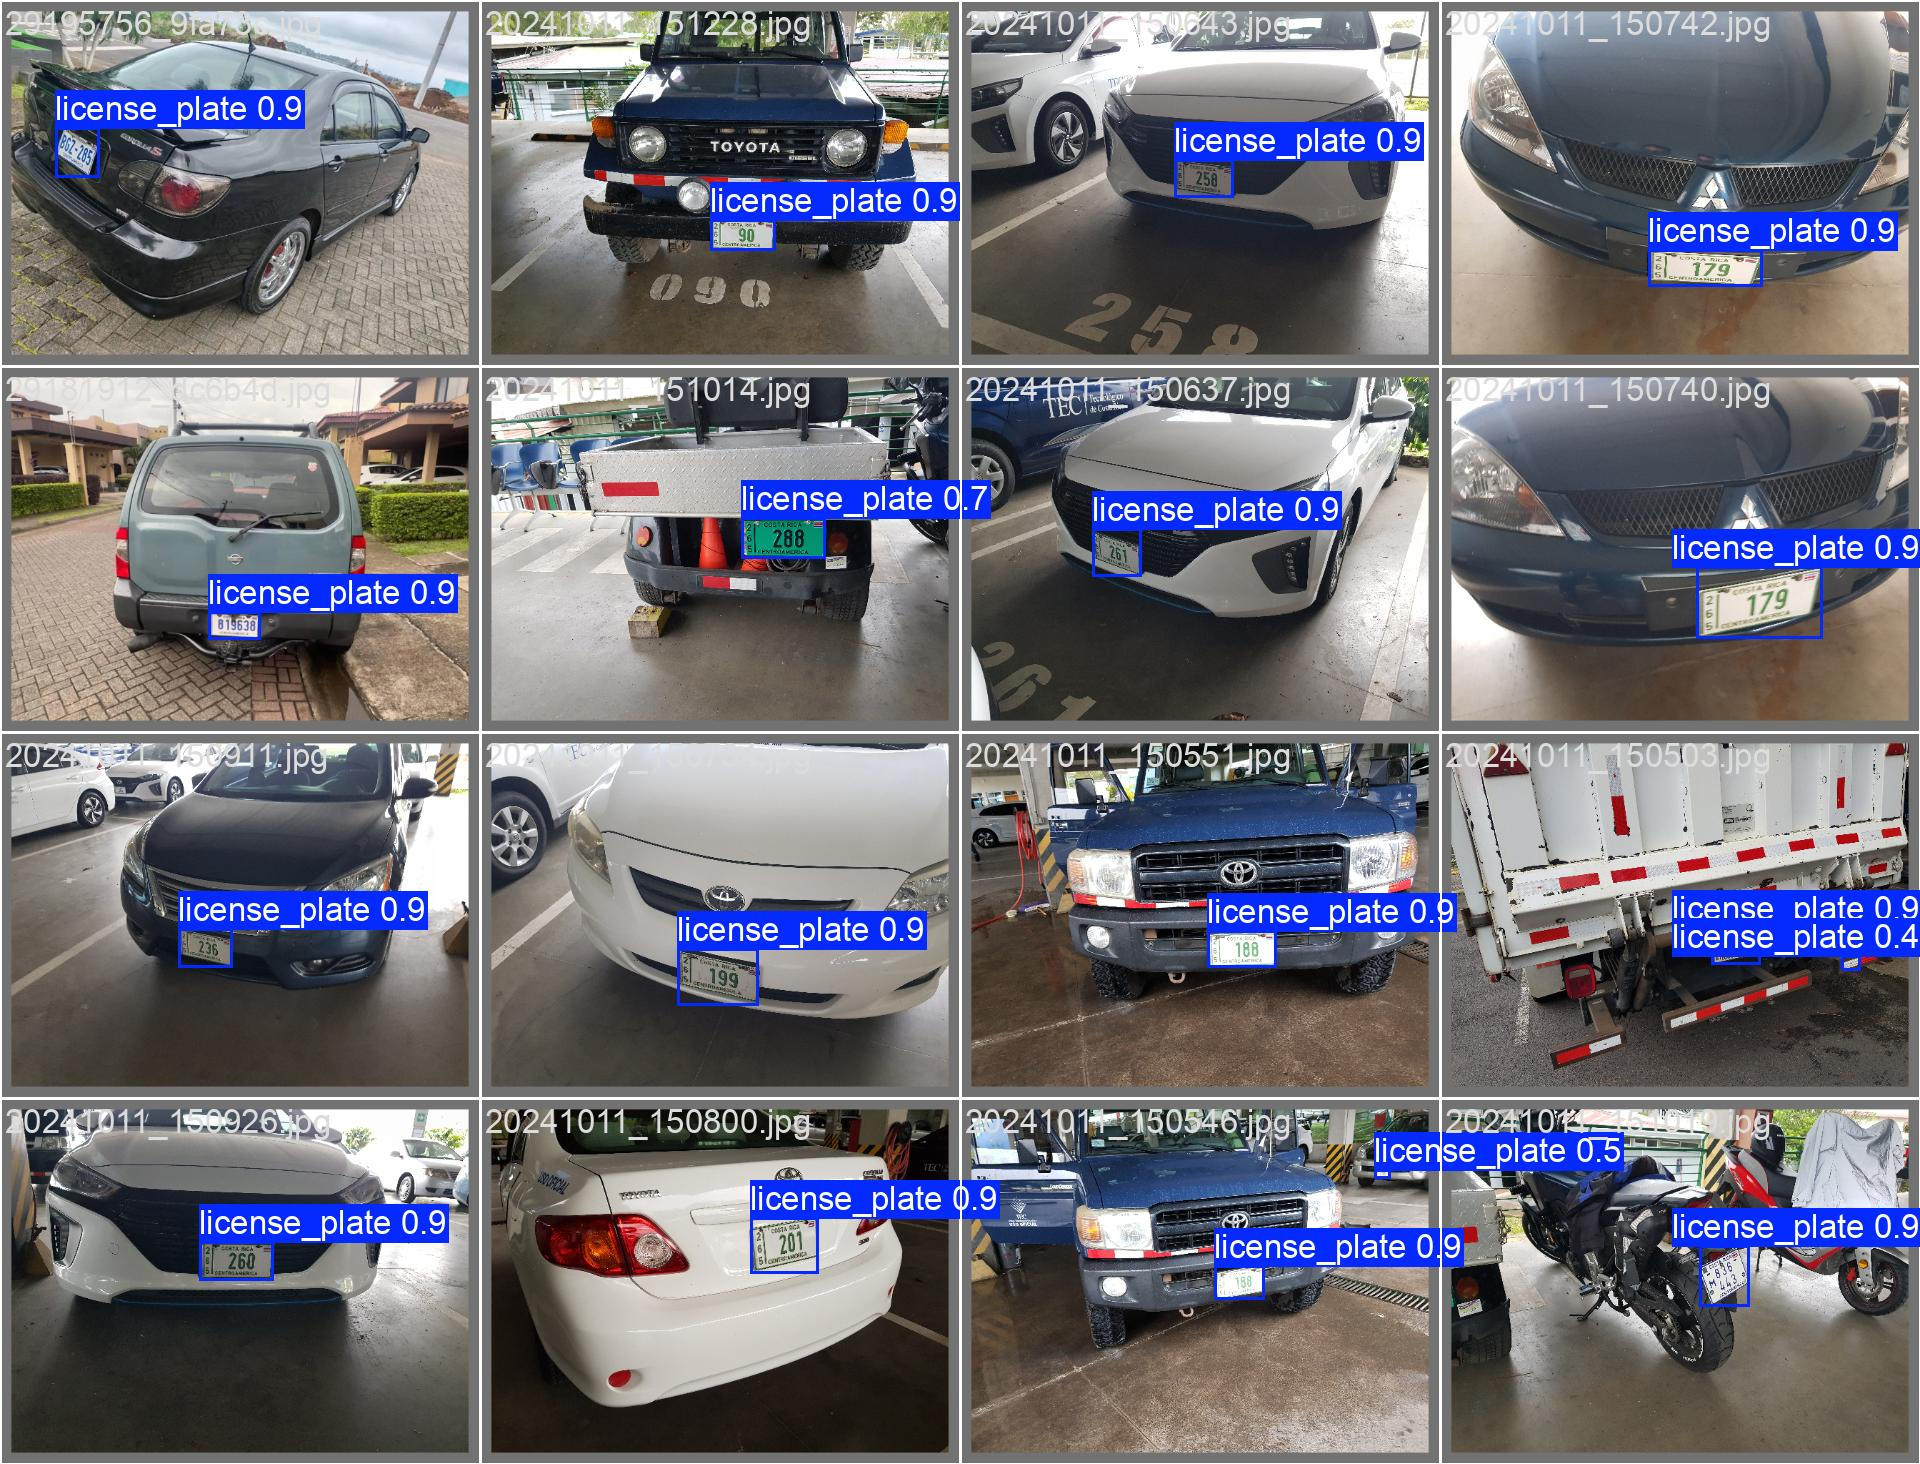
\includegraphics[width=\textwidth]{fig/proy/ejemplo-deteccion-placas.jpg}
	\caption{Ejemplo de detección de placas en imágenes}
	\label{fig:ejemplo-deteccion-placa}
\end{figure}

\begin{figure}[H]
	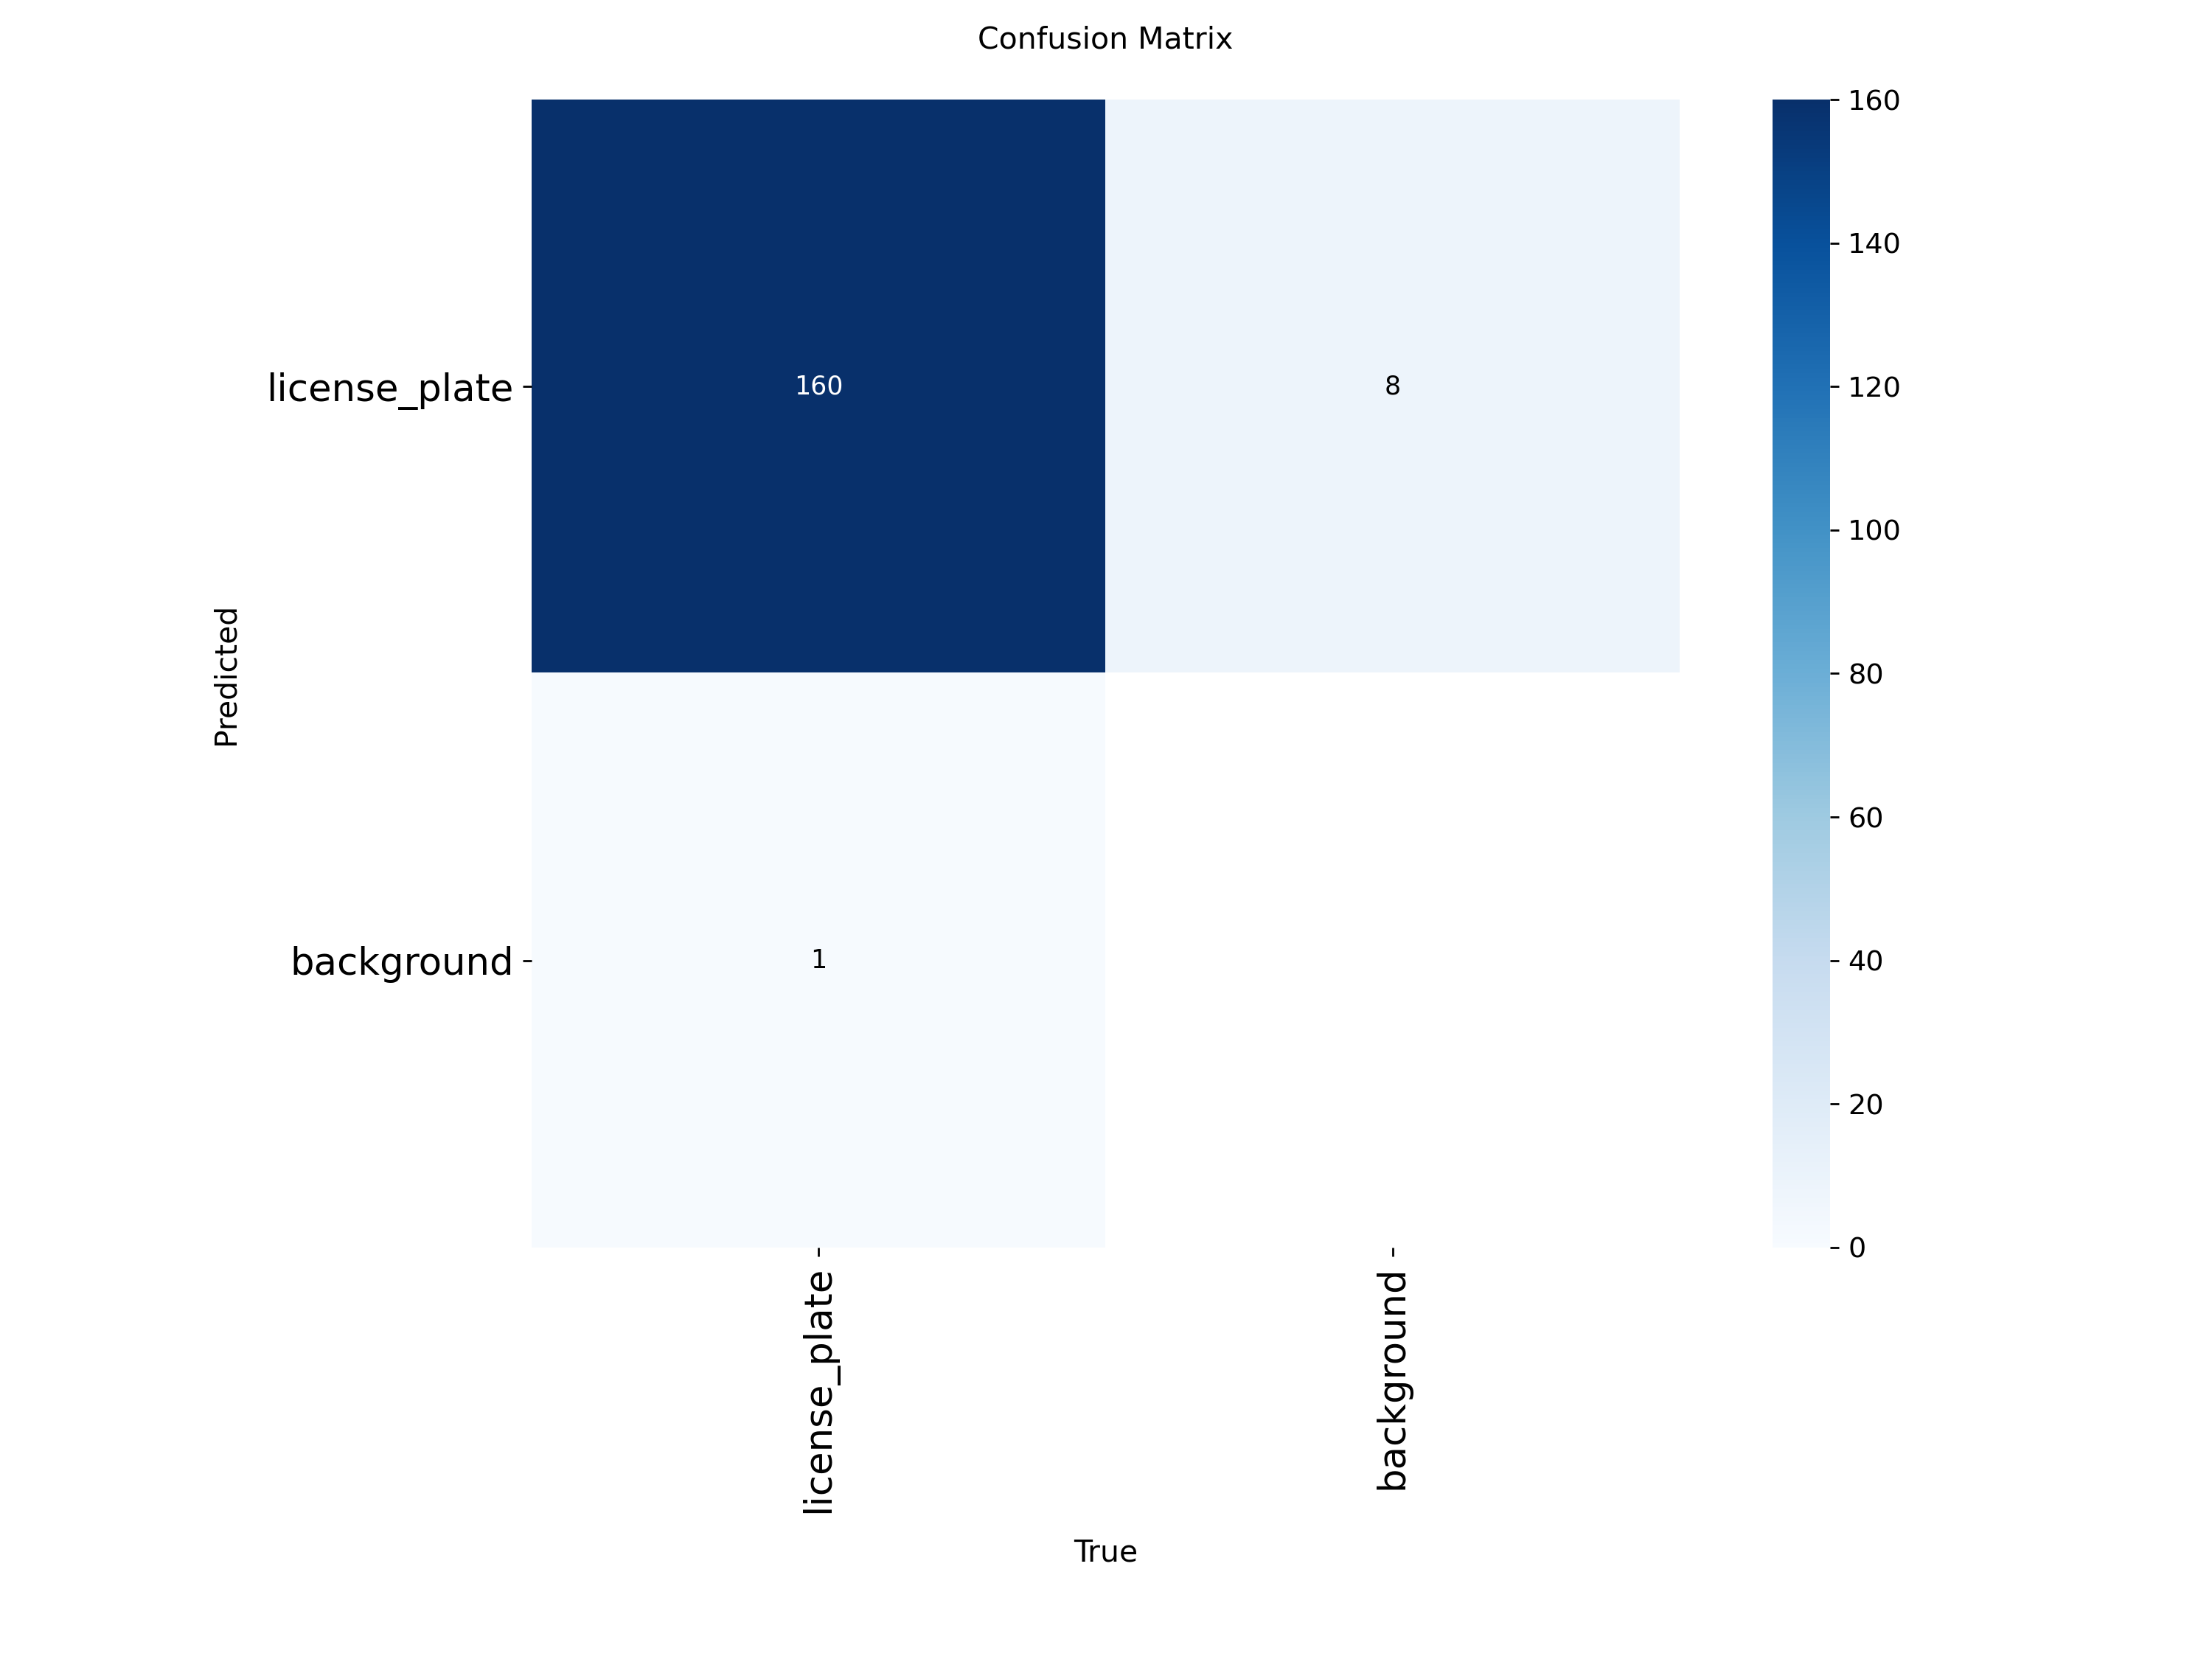
\includegraphics[width=\textwidth]{fig/proy/confusion_matrix-new-model.png}
	\caption{Matriz de confusión del mejor modelo de detección de placas}
	\label{fig:mejor-modelo-yolo}
\end{figure}

En este capítulo se exponen los diseños experimentales realizados para
comprobar el funcionamiento correcto del sistema. Por ejemplo, si se
realiza algún sistema con reconocimiento de patrones, usualmente esta
sección involucra las llamadas \emph{matrices de confusión} donde se
compactan las estadísticas de reconocimiento alcanzadas. En circuitos
de hardware, experimentos para determinar variaciones contra ruido,
etc. También pueden ilustrarse algunos resultados concretos como
ejemplo del funcionamiento de los algoritmos. Puede mostrar por medio
de experimentos ventajas, desventajas, desempeño de su algoritmo, o
comparaciones con otros algoritmos.

Recuerde que debe minimizar los ``saltos'' que el lector deba hacer en
su documento. Por tanto, usualmente el análisis se coloca junto a
\tablas y figuras presentadas, y debe tener un orden de tal modo que se
observe cómo los objetivos específicos y el objetivo general del
proyecto de tesis se han cumplido.

  \chapter{Conclusiones}

Las conclusiones no son un resumen de lo realizado sino a lo que ha llevado el
desarrollo de la tesis, no perdiendo de vista los objetivos planteados desde
el principio y los resultados obtenidos.  En otras palabras, qué se concluye o
a qué se ha llegado después de realizado la tesis de maestría.  Un error
común es ``concluir'' aspectos que no se desarrollaron en la tesis, como
observaciones o afirmaciones derivadas de la teoría directamente.  Esto último
debe evitarse.

Es fundamental en este capítulo hacer énfasis y puntualizar los
aportes específicos del trabajo.

Es usual concluir con lo que queda por hacer, o sugerencias para mejorar los
resultados.



  %----------------------------------------------------------------------------
  % literature in bibtex way:
  % \bibliographystyle{sty/plainurl} % for english documents
  % \bibliography{literatura}
  % literature in biblatex/biber way
  \printbibliography[title={Bibliografía},heading=bibintoc]
  %----------------------------------------------------------------------------

  %----------------------------------------------------------------------------
  \appendix
  %----------------------------------------------------------------------------

  \chapter{Demostración del teorema de Nyquist}
\label{apx:apendice}

El título anterior es solo un ejemplo ilustrativo.  Éste teorema no ameritaría
un apéndice pues es parte normal del currículum de Electrónica, pero apéndices
usualmente involucran aspectos de esta índole, que se salen de la línea de la
tesis, pero que es conveniente incluir por completitud.

Los anexos contienen toda información adicional que se considere pertinente
agregar, como manuales de usuario, demostraciones matemáticas que se salen de
la línea principal de la tesis, pero que pueden considerarse parte de los
resultados del trabajo.


  %----------------------------------------------------------------------------
  \backmatter
  %----------------------------------------------------------------------------

  \printindex                % insert index into document. Don't forget to call
                             % "makeindex filename" first.
\end{document}
